% THIS TEMPLATE IS A WORK IN PROGRESS
% Adapted from an original template by faculty at Reykjavik University, Iceland

\documentclass{scrartcl}
\input{File_Setup.tex}
\usepackage{graphicx,epsfig}
\usepackage{subcaption}
\captionsetup[subfigure]{font=footnotesize}

\usepackage{longtable}
\usepackage{tabularx}
\usepackage{booktabs}
\usepackage{float}
\usepackage{multirow}
\usepackage{tikz}
\usetikzlibrary{arrows.meta, positioning}
\usepackage{adjustbox}
\usepackage{svg}



\hypersetup{
   colorlinks   = true,                               %Colours links instead of ugly boxes
   urlcolor     = blue,                               %Colour for external hyper links
   linkcolor    = blue,                               %Colour of internal links
   citecolor    = red,                                %Colour of citations
   setpagesize  = false,
   linktocpage  = true,
}
\graphicspath{ {fig/} }



\renewenvironment{abstract}{
    \centering
    \textbf{Abstract}
    \vspace{0.5cm}
    \par\itshape
    \begin{minipage}{0.7\linewidth}}{\end{minipage}
    \noindent\ignorespaces
}
% ------------------------------------------------------------------------------------------------------------------------

\begin{document}
%Title of the report, name of coworkers and dates (of experiment and of report).
\begin{titlepage}
	\centering
	\includegraphics[width=0.6\textwidth]{fig/GW_logo-eps-converted-to.pdf}\par
	\vspace{2cm}
	%%%% COMMENT OUT irrelevant lines below: Data Science OR Computer Science OR none
	{\scshape\LARGE Data Science Program \par}
	\vspace{1cm}
	{\scshape\Large Capstone Report - Fall 2025\par}
	%{\large \today\par}
	\vspace{1.5cm}
	%%%% PROJECT TITLE
	{\huge\bfseries Predictive Modeling and Explainable AI for Autism Spectrum Disorder Diagnosis Project\par}
	\vspace{2cm}
	%%%% AUTHOR(S)
	{\Large\itshape Anirudh Rao,\\ Ramana Bhaskar Kosuru,\\ Wilona Nguyen\\}\par
	\vspace{1.5cm}
	supervised by\par
	%%%% SUPERVISOR(S)
	Dr. Amir Jafari
    \\ Dr. Gabriela Rosenblau\\
    \vspace{1.5cm}
	assisted by\par
	Lexie Mathis
    

    \newpage
	\vfill
	\begin{abstract}
	    The diagnosis of Autism Spectrum Disorder (ASD) remains predominantly reliant on subjective clinical judgment, resulting in inconsistencies, delayed detection, and limited generalizability across populations. Addressing this challenge requires the development of interpretable and data-driven diagnostic frameworks that integrate diverse information sources. This study proposes a  machine learning approach that combines behavioral and linguistic data to enhance diagnostic precision and understanding of ASD. By leveraging supervised learning for classification and unsupervised learning for subtype discovery, the framework aims to identify subtle behavioral–linguistic patterns associated with ASD while maintaining model interpretability through explainable AI techniques. Empirical analyses demonstrate that the proposed models outperform traditional single-modality baselines in both diagnostic accuracy and transparency, effectively capturing cross-domain relationships that contribute to ASD heterogeneity. The results highlight the potential of interpretable  models to improve clinical decision-making, foster the discovery of meaningful ASD subtypes, and advance the development of more objective, equitable, and generalizable tools for ASD assessment and research.
	\end{abstract}
	\vfill
% Bottom of the page
\end{titlepage}
\tableofcontents
\newpage
% ------------------------------------------------------------------------------------------------------------------------
\section{Introduction}



Autism Spectrum Disorder (ASD) is a complex neurodevelopmental condition characterized by substantial variability in social communication, behavioral patterns, and cognitive processing. As described by Lord et al.\ \cite{lord2020asd}, ASD encompasses a heterogeneous set of developmental trajectories and phenotypic presentations, with differences observed in social attention, language acquisition, sensory reactivity, adaptive functioning, and co-occurring psychiatric or medical conditions. The disorder arises from multifactorial influences, including diverse genetic architectures and neurobiological pathways, which contribute to the wide range of symptom severity and functional outcomes observed across individuals. This pronounced heterogeneity poses significant challenges for early detection, diagnosis, and personalized intervention, underscoring the need for analytic approaches capable of capturing subtle and multidimensional variation within the spectrum.

Although scientific understanding of ASD has advanced considerably over the past several decades, diagnostic practices remain slow, subjective, and heavily dependent on clinician judgment. Gold-standard assessments, such as the Autism Diagnostic Observation Schedule (ADOS) and the Autism Diagnostic Interview--Revised (ADI--R), require extensive clinical training, rely on behavioral observation, and are often time-consuming to administer. As noted by Yu, Ozonoff, and Miller \cite{yu2024assessment}, these instruments are resource-intensive, can span multiple hours across several sessions, and demand substantial expertise to score and interpret reliably. Moreover, diagnostic evaluations frequently involve long waitlists and limited access to trained specialists, contributing to substantial delays in identification and intervention, particularly for underserved or geographically remote populations. The authors emphasize that diagnostic outcomes are influenced not only by child characteristics but also by examiner experience, contextual factors, and variability in behavioral presentation across settings, further reinforcing the inherent subjectivity of current practices. This combination of logistical burden, variability, and limited scalability highlights the need for complementary computational tools that can support more efficient, accessible, and consistent ASD assessment. 

 As a result of the limitations inherent in current diagnostic practices, there is a widening gap between traditional behavioral assessment methods and the potential of modern computational approaches to improve diagnostic efficiency, objectivity, and scientific understanding of ASD heterogeneity. While gold-standard tools remain indispensable, they were not designed to leverage the depth and breadth of high-dimensional data now available through digital assessments, language sampling, and large-scale research repositories. Consequently, opportunities to detect early markers, quantify nuanced behavioral patterns, and characterize individual differences often remain underrealized. Bridging this gap requires methodological frameworks capable of capturing the complexity of ASD while providing clinically meaningful insights that complement practitioner expertise.

To address these limitations, the present study investigates how interpretable,  machine learning models can enhance both the diagnostic precision and conceptual understanding of ASD. Rather than relying exclusively on structured clinical indicators, this work incorporates richer behavioral and linguistic signals that reflect real-world cognitive and social processes. By doing so, the study seeks to evaluate whether  modeling can more accurately differentiate ASD from typically developing (TD) populations and whether interpretability techniques can surface the underlying behavioral constructs that drive model predictions.

Central to this investigation is the integration of behavioral and linguistic data sources, which allows the analysis to move beyond traditional single-modality assessments toward more objective, data-driven diagnostic frameworks. Behavioral metrics capture observable features of task performance, while natural language responses provide a unique window into narrative coherence, inferential reasoning, and pragmatic communication—domains known to vary meaningfully across the autism spectrum. The combined use of these modalities enables the identification of subtle behavioral–linguistic interactions that may be overlooked in structured instruments but are highly relevant to ASD characterization.

The proposed machine learning pipeline employs a combination of supervised and unsupervised learning techniques to advance both prediction and discovery. XGBoost is utilized as the core classifier due to its strong performance with heterogeneous feature sets and its compatibility with post-hoc interpretability frameworks. Dimensionality reduction and clustering methods—including PCA, KMeans, t-SNE, and HDBSCAN—are applied to uncover latent structure, visualize high-dimensional relationships, and identify potential ASD subtypes. These algorithms collectively support a rigorous exploration of the data, ensuring that observed patterns are not merely artifacts of a single modeling strategy but reflect consistent trends across analytical methods.

Ultimately, this study contributes to the development of transparent, generalizable, and equitable computational tools that advance ASD diagnosis, subtype discovery, and data-informed clinical decision-making. By using explainable artificial intelligence (XAI) methods such as SHAP and LIME, the models provide clear, interpretable explanations that can help clinicians understand why specific predictions are made, fostering trust and facilitating responsible clinical integration. Moreover, the integration of clustering-based subtype exploration reflects a step toward more personalized assessments that recognize the diversity of ASD manifestations. Collectively, these advances position computational methods not as replacements for clinical expertise but as powerful complements that enhance the precision, scalability, and scientific depth of ASD evaluation.






% ------------------------------------------------------------------------------------------------------------------------
\section{Problem Statement}
Recent developments in machine learning (ML) have demonstrated promising results in ASD prediction, with some studies achieving strong classification performance using structured behavioral, cognitive, or physiological features. Despite these advances, current research still faces critical limitations that constrain real-world clinical applicability. 

First, the majority of ASD classification studies rely on structured data such as questionnaire scores, psychometric assessments, or task-based behavioral metrics. While these approaches have yielded promising predictive performance, they largely overlook unstructured linguistic information, including free-text responses elicited during social inference tasks, narrative retellings, or open-ended interviews. Such linguistic data capture a broad spectrum of expressive and cognitive processes, encompassing coherence and narrative structure, abstraction and inferencing ability, pragmatic language use, semantic richness, and the organization of social-cognitive reasoning. A substantial body of clinical and developmental research has shown that these linguistic dimensions often differ systematically between individuals with ASD and typically developing (TD) populations. Despite this, they have seen limited incorporation into computational pipelines, which tend to favor predefined, instrument-based features.

The underutilization of unstructured text represents a missed opportunity, as language provides a naturalistic and highly sensitive window into social understanding, perspective-taking, and cognitive style—domains that are central to ASD characterization. Moreover, free-text responses allow individuals to articulate thoughts in their own words, offering far richer and more individualized signals than fixed-choice questionnaire items. Advances in natural language processing (NLP) and language-model-based feature extraction now make it feasible to analyze these nuanced linguistic patterns at scale, yet integration of such methods remains rare in ASD machine learning research. As a result, current models risk overlooking meaningful markers of social-cognitive reasoning that cannot be captured through traditional structured assessments alone.

Second, while ML models frequently achieve high predictive accuracy, many operate as opaque ``black boxes,'' providing minimal insight into the internal mechanisms driving their predictions. This opacity poses a substantial barrier to clinical adoption, as clinicians and researchers must be able to understand why a model arrives at a given decision in order to evaluate its reliability, assess potential biases, and integrate its output into diagnostic reasoning. In high-stakes domains such as ASD assessment, predictions that lack transparency are difficult to validate and may undermine practitioner trust, even when numerical performance metrics are strong. Moreover, without interpretable explanations, it is challenging to determine whether a model is relying on clinically meaningful behavioral or cognitive indicators, or instead exploiting dataset-specific artifacts that fail to generalize. Although emerging Explainable Artificial Intelligence (XAI) techniques such as SHAP and LIME offer mechanisms to characterize global feature importance and provide case-level interpretability, these tools are still rarely integrated into ASD-focused classification pipelines. As a result, much of the existing literature continues to favor predictive accuracy over interpretive clarity, limiting the feasibility of real-world clinical integration.

Third, although ASD is inherently heterogeneous, most computational studies continue to treat it as a single monolithic diagnostic category. This oversimplification obscures meaningful intra-group variability in linguistic expression, cognitive strategies, social-communicative patterns, sensory-motor behaviors, and developmental pathways. As a result, important subpopulations within the autism spectrum---such as individuals with distinct language profiles, compensatory strategies, or behavioral phenotypes---are collapsed into a single label, limiting the scientific and clinical insights that ML models can provide. Unsupervised learning techniques, including clustering, dimensionality reduction, and manifold learning, offer powerful tools for uncovering latent ASD subtypes that may reflect real neurocognitive or behavioral distinctions. Identifying these subgroups could support more accurate diagnosis, earlier detection of high-risk phenotypes, and personalized intervention strategies tailored to individual needs. Despite this potential, such methods remain underexplored in current autism research, where the emphasis continues to fall disproportionately on binary ASD vs.\ TD classification rather than understanding within-spectrum heterogeneity.

Finally, the generalizability of ASD classification models across diverse datasets, tasks, and participant groups is seldom evaluated. Many studies validate their models exclusively on a single dataset collected under highly controlled conditions, which limits the robustness, reproducibility, and clinical reliability of the findings. Without systematic cross-dataset validation, it is difficult to determine whether models are learning genuine ASD-related patterns or merely overfitting to idiosyncrasies of a particular sample, instrument, or study population. Large-scale, well-curated datasets provided by the Simons Foundation Autism Research Initiative (SFARI)---including SPARK, the Simons Simplex Collection (SSC), and Simons Searchlight---offer unparalleled opportunities for developing models with greater ecological validity. These datasets capture extensive genetic, behavioral, cognitive, and phenotypic information across tens of thousands of families. However, they remain significantly underutilized for advanced ML research, particularly in the context of explainable and multimodal modeling. Leveraging these resources would enable more rigorous evaluation of generalizability, facilitate model replication across heterogeneous cohorts, and support the development of clinically trustworthy ASD prediction frameworks.

% ------------------------------------------------------------------------------------------------------------------------
\section{Related Work}



The majority of ASD classification studies rely on structured data such as questionnaire scores, psychometric assessments, or task-based behavioral metrics. For example, in one study, the data used is limited to structured behavioral instruments such as the ADI--R and SRS \cite{Bone2016MLAutismScreening}. While the authors demonstrate that a reduced subset of questionnaire items can still achieve strong classification performance, the approach remains constrained to traditional psychometric inputs. Their models achieved high accuracy using fewer ADI--R items and showed improvements through multi-instrument fusion, but the predictive signals were still derived entirely from predefined diagnostic checklists. 

Another example comes from a study that uses data from the Autism Genetic Resource Exchange (AGRE) repository, where the data is also primarily composed of structured clinical and behavioral assessments \cite{thabtah2017}. The author applied machine learning methods to AGRE variables such as diagnostic codes, family history, and standardized behavioral ratings to predict ASD risk within multiplex families. Although the study shows that these structured features can yield reasonable predictive performance, the scope of the input data remains restricted to predefined clinical attributes. This further illustrates that much of the existing ASD classification literature relies heavily on structured datasets, in contrast to our approach, which incorporates both structured behavioral metrics and unstructured free-text responses to capture a broader and more nuanced representation of social--cognitive functioning.

These approaches largely overlook unstructured linguistic information, including free-text responses produced during social inference or narrative tasks. Such linguistic data contain rich cues related to coherence, abstraction, pragmatic reasoning, and semantic organization---all of which are known to differ between ASD and typically developing (TD) populations. However, these subtle yet informative patterns remain significantly underutilized in computational ASD research.




% ------------------------------------------------------------------------------------------------------------------------

\section{Solution and Methodology}

\subsection{Dataset Overview}
[Need description of the data]

Data V1 is the Trial Level data. [Need description of the data]

Data V2 is based on Data V1 to compute avg\_PE across each profile. [Need description of the data]

Data V3 is based on Data V2 to compute concept\_learning for each subject across all profiles. [Need description of the data]

\subsubsection{Data Dictionary}

\begin{table}[H]
\centering
\small   % makes the whole table smaller
\caption{Data Dictionary for All Datasets}
\begin{tabular}{|l|l|p{9cm}|}
\hline
\textbf{Data Version} & \textbf{Column Name} & \textbf{Description} \\ \hline

V1, V2, V3 & sub & Participant ID \\ \hline

V1, V2 & subject & Participant ID followed by a random code for the current profile \\ \hline

V1, V2, V3 & td\_or\_asd & Diagnostic group (0 = TD, 1 = ASD) \\ \hline

V1 & asd\_diagnosis\_text & Which ASD diagnosis does the participant have? \\ \hline

V1 & trial & The trial number (1-60)  within the current profile. \\ \hline

V1, V2 & profile & Peer profile (TDprof\_norm, ASDprof\_norm, ASDprof\_unif) \\ \hline

V1 & image & The image shown on the current trial. Order is randomized within profile for each participant.  \\ \hline

V1 & cat & Image category  (1 = activities, 3 = foods) \\ \hline

V1 & subcat & Image subcategory (1 = arts \& crafts, 2 = music \& instruments, 3 = sports, 4 = games \& gadgets, 9 = fast food, 10 = fruits \& vegetables, 11 = healthy \& savory, 12 = desserts) \\ \hline

V1 & concept & Descriptive image concept label \\ \hline

V1 & cnum & Image concept number \\ \hline

V1 & selfpref & How much does the participant like this image? \\ \hline

V1 & asd\_meanpref & On average, how much do ASD participants like this image?  \\ \hline

V1 & td\_meanpref & On average, how much do TD participants like this image?  \\ \hline

V1 & slider\_rating & The participant's rating of how much they think the peer in question like the image shown. \\ \hline

V1 & profile\_rating & The correct rating for the given image and profile (this is the feedback given to participants) \\ \hline

V1 & PE & The absolute difference between a participant's rating of how much they think the peer likes an item and the peer's actual liking of the item (actual liking = feedback). \\ \hline

V1, V2 & avg\_PE or profile\_avg\_PE & Average prediction error on each peer profile \\ \hline

V1 & free\_response & Participant's free response -- what they think about the peer they just learned about. \\ \hline


V2, V3 & SRS.Raw & Raw SRS-2 social responsiveness score (higher = more difficulties) \\ \hline

V2, V3 & FSR & Flexibility Scale-Revised score (higher = less flexibility) \\ \hline

V2, V3 & BIS & Behavioral Inflexibility Scale score (higher = less flexibility) \\ \hline


V1, V2 & free\_response & Participant’s free-text description of the peer \\ \hline

V2 & LPA\_Profile\_grand\_mean & Latent profile (grand-mean centered) \\ \hline

V2 & LPA\_Profile\_ASD\_only & Latent profile (ASD-only analysis) \\ \hline

V3 & TDNorm\_avg\_PE & Across all trials, average PE for TDNorm profile \\ \hline

V3 & overall\_avg\_PE & Across all trials, average PE for all three profiles \\ \hline

V3 & TDNorm\_concept\_learning & Across all trials, slope of PE for TDNorm profile \\ \hline

V3 & overall\_concept\_learning & Across all trials, slope of PE across all three profiles \\ \hline

V3 & free\_response\_TDprof\_norm & Free response text from TDprof\_norm profile \\ \hline

V3 & free\_response\_ASDprof\_norm & Free response text from ASDprof\_norm profile \\ \hline

V3 & free\_response\_ASDprof\_unif & Free response text from ASDprof\_unif profile \\ \hline

\end{tabular}
\end{table}

\subsubsection{Exploratory Data Analysis}
 Table~\ref{tab:dtype} shows the data types for the features in all data versions. The trial level data (Data V1) has 187,187 rows with 19 columns. Data V2 has 2,647 rows and 11 columns. Data V3 has 1,119 rows and 12 columns. 

\begin{table}[H]
\centering
\caption{Data Types}
\renewcommand{\arraystretch}{1.1}

\begin{minipage}{0.32\linewidth}
\centering
\textbf{Data V1} \\[3pt]
\small
\adjustbox{max width=\linewidth}{
\begin{tabular}{l l}
\toprule
Column & Type \\
\midrule
sub & object \\
subject & object \\
td\_or\_asd & int64 \\
asd\_diagnosis\_text & object \\
trial & int64 \\
profile & object \\
image & object \\
cat & int64 \\
subcat & int64 \\
concept & object \\
cnum & int64 \\
selfpref & float64 \\
asd\_meanpref & float64 \\
td\_meanpref & float64 \\
slider\_rating & int64 \\
profile\_rating & int64 \\
PE & int64 \\
profile\_avg\_PE & float64 \\
free\_response & object \\
\bottomrule
\end{tabular}}
\end{minipage}
\hfill
\begin{minipage}{0.32\linewidth}
\centering
\textbf{Data V2} \\[3pt]
\small
\adjustbox{max width=\linewidth}{
\begin{tabular}{l l}
\toprule
Column & Type \\
\midrule
sub & object \\
profile & object \\
subject & object \\
td\_or\_asd & int64 \\
SRS.Raw & float64 \\
FSR & float64 \\
BIS & float64 \\
avg\_PE & float64 \\
free\_response & object \\
LPA\_Profile\_grand\_mean & int64 \\
LPA\_Profile\_ASD\_only & float64 \\
\bottomrule
\end{tabular}}
\end{minipage}
\hfill
\begin{minipage}{0.32\linewidth}
\centering
\textbf{Data V3} \\[3pt]
\small
\adjustbox{max width=\linewidth}{
\begin{tabular}{l l}
\toprule
Column & Type \\
\midrule
sub & object \\
td\_or\_asd & int64 \\
FSR & float64 \\
BIS & float64 \\
SRS.Raw & int64 \\
TDNorm\_avg\_PE & float64 \\
overall\_avg\_PE & float64 \\
TDnorm\_concept\_learning & float64 \\
overall\_concept\_learning & float64 \\
free\_response\_TDprof\_norm & object \\
free\_response\_ASDprof\_norm & object \\
free\_response\_ASDprof\_unif & object \\
\bottomrule
\end{tabular}}
\end{minipage}

\label{tab:dtype}
\end{table}





Figure~\ref{fig:eda1-all} summarizes the distribution of some key categorical features used in the trial-level dataset. Panel~\subref{fig:eda1-profiles} shows the profile variable, which consists of three experimental profile types (TDprof\_norm, ASDprof\_unif, and ASDprof\_norm) with broadly comparable frequencies, each appearing roughly between 61{,}000 and 63{,}000 times. This indicates that the profiling procedure was applied in a relatively balanced way across the different profile conditions, which helps reduce potential confounding due to uneven exposure to specific profile types. Panel~\subref{fig:eda1-diag} displays the binary td\_or\_asd label, revealing a moderate class imbalance, with one group represented in approximately 115{,}970 trials and the other in about 71{,}217 trials.

Panel~\subref{fig:eda1-asd-diag} further refines the diagnostic information by breaking the ASD group into specific diagnostic categories based on the asd\_diagnosis\_text field. The majority of ASD trials are associated with the “Autism” label (over 100{,}000 observations), followed by smaller but still substantial counts for “Aspergers Disorder”; rarer categories such as “PDD-NOS”, “Child Disintegrative Disorder (CDD)”, and “Other or Unknown” are present in much lower frequencies. This long-tailed distribution suggests that while the dataset provides rich coverage for core autism diagnoses, analyses focusing on rarer ASD subtypes may require additional care (for example, aggregation or hierarchical modeling) to avoid unstable estimates. Panel~\subref{fig:eda1-cat} shows the high-level category variable \texttt{cat}, which contains only two codes with relatively similar but not identical frequencies (roughly 99{,}835 vs.\ 87{,}352).This indicates that participants are exposed to two broad task or stimulus categories at a scale that is reasonably balanced, supporting comparisons across these top-level conditions.




\vspace{0.5cm}

\begin{figure}[H]
\centering

% ----- Row 1 -----
\begin{subfigure}{0.45\textwidth}
    \centering
    \includegraphics[width=\textwidth]{fig/eda/data v1/profile_eda_plot.pdf}
    \caption{Profiles}
    \label{fig:eda1-profiles}
\end{subfigure}
\hfill
\begin{subfigure}{0.45\textwidth}
    \centering
    \includegraphics[width=\textwidth]{fig/eda/data v1/td_or_asd_eda_plot.pdf}
    \caption{Diagnosis}
    \label{fig:eda1-diag}
\end{subfigure}

\vspace{0.4cm}

% ----- Row 2 -----
\begin{subfigure}{0.45\textwidth}
    \centering
    \includegraphics[width=\textwidth]{fig/eda/data v1/asd_diagnosis_text_eda_plot.pdf}
    \caption{ASD Diagnosis}
    \label{fig:eda1-asd-diag}
\end{subfigure}
\hfill
\begin{subfigure}{0.45\textwidth}
    \centering
    \includegraphics[width=\textwidth]{fig/eda/data v1/cat_eda_plot.pdf}
    \caption{Categories}
    \label{fig:eda1-cat}
\end{subfigure}

\vspace{0.4cm}

% ----- Row 3 -----
\begin{subfigure}{0.45\textwidth}
    \centering
    \includegraphics[width=\textwidth]{fig/eda/data v1/subcat_eda_plot.pdf}
    \caption{Sub-Categories}
    \label{fig:eda1-subcat}
\end{subfigure}
\hfill
\begin{subfigure}{0.45\textwidth}
    \centering
    \includegraphics[width=\textwidth]{fig/eda/data v1/concept_eda_plot.pdf}
    \caption{Concepts}
    \label{fig:eda1-concepts}
\end{subfigure}

\caption{Distribution of Some Features in Data V1}
\label{fig:eda1-all}
\end{figure}

Panel~\subref{fig:eda1-subcat} shows the subcat feature, which comprises eight distinct subcategory codes with varying frequencies ranging from around 11{,}441 to over 31{,}000 trials. Although some subcategories are more frequently sampled than others, all codes are represented with sufficient counts to support subcategory-level analyses if desired. Finally, Panel~\subref{fig:eda1-concepts} illustrates the concept variable, capturing 25 distinct semantic concepts such as “games”, “baked\_goods”, “fruit”, “instrument”, and “fast\_food”. The distribution is heterogeneous: a few concepts appear very frequently (e.g., “games”, “baked\_goods”), while many others have mid-range counts in the 3{,}000–12{,}000 range. This diversity in concept-level stimuli is valuable for downstream modeling, as it provides a rich set of semantic contexts for probing differences between ASD and TD groups while still maintaining adequate sample sizes per concept for robust estimation.

%corr-heat
\begin{figure}[H]
    \centering
    \includesvg[width=0.9\linewidth]{fig/eda/corr-heat.svg}
    \caption{Correlation Heatmap}
    \label{fig:corr-heat}
\end{figure}


The correlation heatmap in Figure~\ref{fig:corr-heat} provides an overview of relationships among all behavioral, concept-learning, and linguistic features. As expected, several behavioral measures exhibit strong inter-correlations (e.g., FSR, BIS, and SRS-Raw), reflecting overlapping constructs within ASD-related assessments. Notably, SRS-Raw shows an extremely high correlation with the target label, indicating clear target leakage, and therefore must be excluded from all predictive modeling. Linguistic variables mostly display weak to moderate correlations with behavioral metrics, suggesting that they capture complementary rather than redundant information. Together, these results help justify our feature-selection decisions and highlight which variables require careful handling before model training.


%--------------------------------------------------------------------------------------------------------------------

\subsection{Project Pipeline}

The project develops an end-to-end machine learning pipeline that extracts insights from unstructured text, integrates behavioral metrics, and builds interpretable ASD versus TD classification models.

\vspace{0.5cm}

\begin{figure}[ht]
\centering
\resizebox{0.9\linewidth}{!}{%
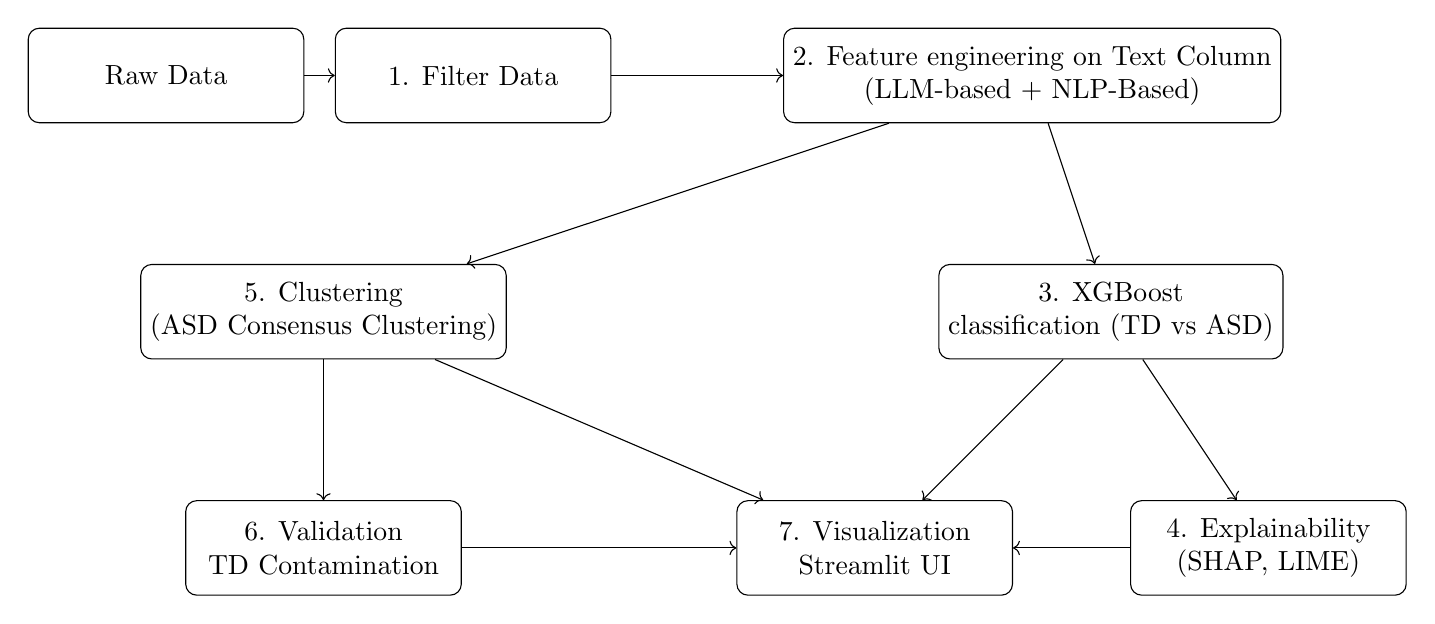
\begin{tikzpicture}[
    block/.style = {
        rectangle,
        rounded corners,
        draw,
        align=center,
        minimum height=1.2cm,
        minimum width=3.5cm
    }
]

% Nodes with explicit coordinates
\node[block] (raw)  at (0,0)   {Raw Data};
\node[block] (pre)  at (3.9,0)   {1. Filter Data};
\node[block] (feat) at (11,0)   {2. Feature engineering on Text Column\\(LLM-based + NLP-Based)};

\node[block] (cluster) at (2,-3)  {5. Clustering\\ (ASD Consensus Clustering)};
\node[block] (contam) at (2,-6)  {6. Validation \\ TD Contamination};
\node[block] (xgb)     at (12,-3)  {3. XGBoost\\classification (TD vs ASD)};
\node[block] (xai)     at (14,-6) {4. Explainability\\(SHAP, LIME)};

\node[block] (ui)      at (9,-6)  {7. Visualization\\Streamlit UI};

% Arrows (main pipeline)
\draw[->] (raw) -- (pre);
\draw[->] (pre) -- (feat);
\draw[->] (feat) -- (xgb);
\draw[->] (feat) -- (cluster);

% Branches from classifier
\draw[->] (xgb) -- (xai);
\draw[->] (xgb) -- (ui);

% Send clustering and XAI results to UI
\draw[->] (contam) -- (ui);
\draw[->] (cluster) -- (ui);
\draw[->] (xai) -- (ui);

\draw[->] (cluster) -- (contam);

\end{tikzpicture}

} % end resizebox
\caption{Pipeline diagram.}
\label{fig:pipeline}
\end{figure}

As illustrated in Figure~\ref{fig:pipeline}, the entire workflow forms an end-to-end machine learning system that integrates text preprocessing, LLM and NLP based feature engineering, supervised classification, model interpretability, unsupervised consensus clustering, and cluster validation . Raw free-response text is first cleaned and standardized before being transformed into high-dimensional semantic representations using LLM agents such as Anthropic Sonnet, Qwen, and HuggingFace Llama. NLP based features like counts, polarities etc are derived from the free-response text using libraries like NLTK and TextBlob. These engineered features are then merged with behavioral and concept-learning measures and fed into an XGBoost classifier to distinguish Autism Spectrum Disorder (ASD) from Typically Developing (TD) participants. Finally, explainable AI methods, including SHAP and LIME, are applied to quantify feature importance and provide interpretable insights into classification components. For ASD subtype analysis, consensus clustering is employed which is then statistically validated and followed by TD imputation to understand if there is truth to the cluster formation.

\subsubsection{Text Data Preprocessing}

As shown in Figure \ref{fig:dataprep-pipe}, the preprocessing pipeline begins by loading the aggregated dataset containing participant identifiers, behavioral metrics, concept-learning scores, and free-response text. A curated subset of relevant variables is selected, and rows with missing values are removed to ensure that downstream models operate on complete, high-quality data. Metadata about the preprocessing step—including original and filtered shapes, selected variables, and the target label distribution—is stored for reproducibility and experiment tracking. The dataset is then split into training and testing sets using a stratified sampling strategy that preserves the original class proportions, ensuring balanced evaluation across ASD and TD groups.

After structural filtering, the pipeline performs natural language feature engineering on the cleaned free-response text. Each response is normalized and tokenized using NLTK, with operations that include lowercasing, word tokenization, sentence segmentation, stop-word removal, and optional lemmatization. The system computes a comprehensive set of linguistic features that characterize the text at multiple levels \cite{nltk}. Basic descriptive statistics—such as word count, character count, number of sentences, average word length, and average sentence length—capture surface-level linguistic production patterns. Additional stylistic constructs include a shortness score, which emphasizes concise responses, and lexical diversity, which measures the proportion of unique words relative to total word usage.

To further enrich the text representation, the pipeline extracts affective and sentiment-based features. Using TextBlob, each response is assigned polarity and subjectivity scores that quantify emotional tone and expressive style \cite{textblob}. The pipeline additionally identifies predefined sets of positive and negative lexical items (e.g., love, good, hate, don’t) and computes their counts and ratios within the response. These ratios help capture implicit preferences and aversions expressed in the free-response text. Readability metrics, including Flesch Reading Ease and Flesch–Kincaid grade level, are computed to reflect the cognitive and linguistic complexity of each response, providing another dimension of variation that may correlate with participant group patterns.

% \vspace{0.5cm}
% \begin{figure}[ht]
% \centering

% \begin{tikzpicture}[
%     node distance=1.4cm,
%     box/.style={
%         rectangle,
%         draw,
%         rounded corners,
%         align=center,
%         minimum width=6cm,
%         minimum height=1.1cm,
%         fill=gray!10
%     },
%     arrow/.style={-Stealth, thick}
% ]

% \node[box] (load) {Dataset};
% \node[box, below=of load] (filter) {Filter ASD};
% \node[box, below=of filter] (cor) {Correlation Elimination};
% \node[box, below=of cor] (vif) {VIF Elimination};
% \node[box, below=of vif] (cc) {Consensus Clustering};
% \node[box, below=of cc] (eval) {Best K evaluation};
% \node[box, below=of eval] (val) {Statistical Validation};
% \node[box, below=of val] (contam) {TD Contamination};
% \node[box, below=of contam] (conclusions) {Conclusions};

% \draw[arrow] (load) -- (filter);
% \draw[arrow] (filter) -- (cor);
% \draw[arrow] (cor) -- (vif);
% \draw[arrow] (vif) -- (cc);
% \draw[arrow] (cc) -- (eval);
% \draw[arrow] (eval) -- (val);
% \draw[arrow] (val) -- (contam);
% \draw[arrow] (contam) -- (conclusions);

% \end{tikzpicture}

% \caption{Overview of the clustering pipeline.}
% \label{fig:dataprep-pipe}
% \end{figure}

\vspace{0.5cm}
\begin{figure}[ht]
\centering

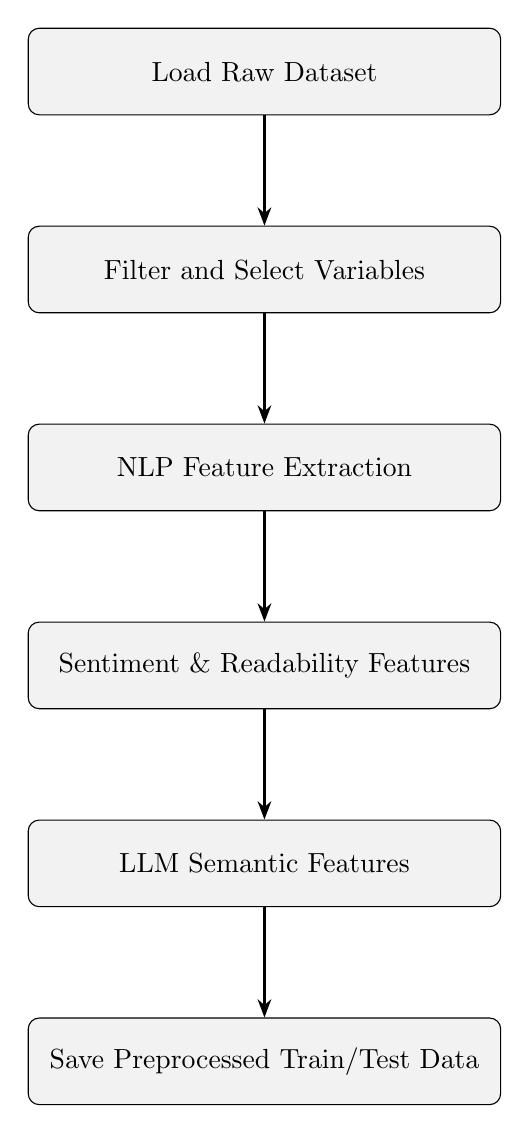
\begin{tikzpicture}[
    node distance=1.4cm,
    box/.style={
        rectangle,
        draw,
        rounded corners,
        align=center,
        minimum width=6cm,
        minimum height=1.1cm,
        fill=gray!10
    },
    arrow/.style={-Stealth, thick}
]

\node[box] (load) {Load Raw Dataset};
\node[box, below=of load] (filter) {Filter and Select Variables};
\node[box, below=of filter] (nlp) {NLP Feature Extraction};
\node[box, below=of nlp] (sentiment) {Sentiment \& Readability Features};
\node[box, below=of sentiment] (llm) {LLM Semantic Features};
\node[box, below=of llm] (save) {Save Preprocessed Train/Test Data};

\draw[arrow] (load) -- (filter);
\draw[arrow] (filter) -- (nlp);
\draw[arrow] (nlp) -- (sentiment);
\draw[arrow] (sentiment) -- (llm);
\draw[arrow] (llm) -- (save);

\end{tikzpicture}

\caption{Overview of the data preprocessing pipeline.}
\label{fig:dataprep-pipe}
\end{figure}



\subsubsection{Features Engineering}

To incorporate qualitative behavioral information, free-text responses are converted into quantitative features using a custom NLPFeatureExtractor built with NLTK, TextBlob, and textstat. The extractor generates several categories of linguistic features that capture length, structure, sentiment, vocabulary richness, and readability.

First, basic length and structural features are computed, including word count, sentence count, character count, average word length, and average sentence length measured as the number of words per sentence. These features help characterize the general verbosity or conciseness of a participant’s written response.

A shortness score is also included to capture extremely brief responses. This metric, calculated as 1 divided by (1 + word count), increases as the response becomes shorter and serves as a simple indicator of minimal engagement or a terse writing style.

Lexical variety is quantified using lexical diversity, defined as the ratio of unique words to total words. This provides a measure of vocabulary richness and helps distinguish repetitive or low-variety writing from more expressive responses.

Sentiment features are extracted using TextBlob, producing numerical estimates of polarity (positive vs. negative sentiment) and subjectivity (objective vs. subjective tone). These help capture the emotional framing and personal perspective embedded in the text.

To more directly quantify emotional language, the extractor counts the number of positive and negative words using curated lexicons. It also computes ratios that normalize these counts by total words, providing scale-invariant measures of positive or negative word usage.

Readability metrics are computed using textstat, including Flesch Reading Ease and Flesch–Kincaid Grade Level. These scores approximate the linguistic complexity of the response. If the library fails to compute a value, a default value of zero is used to ensure consistency.

The architecture also includes  high-level semantic analysis using an LLM-based characteristic feature extractor (Optional - Not used in later versions of modeling). When enabled, this module loads a predefined list of behavioral and conceptual characteristics from a text file and constructs a structured system prompt that instructs the LLM to detect whether each characteristic is mentioned or implied within the participant’s free-response text. For every response, the LLM returns a JSON-formatted analysis specifying three attributes for each characteristic: whether it is mentioned, and whether the expressed sentiment is positive, negative, or neutral. The pipeline converts these outputs into machine-learning features by creating indicator variables such as \_mentioned, \_positive, \_negative, and \_neutral for each characteristic. Robust error handling ensures that malformed or non-JSON responses are safely corrected or replaced with neutral defaults, and a logging system records any failed samples for auditing. This LLM-driven semantic extraction provides a high-level conceptual representation of participants’ reasoning styles, preferences, and cognitive framing that extends beyond what traditional NLP statistics can capture.

Once all NLP and LLM-based features are extracted, they are appended to the dataset, substantially expanding the original set of variables. The enriched training and testing datasets are then saved to disk with version-controlled filenames, ensuring repeatability and streamlined integration with the subsequent classification and clustering stages. By consolidating text normalization, linguistic feature engineering, semantic extraction, and reproducible data handling, the preprocessing pipeline establishes a consistent foundation for all models and experiments in the workflow.

\subsubsection{XGBoost Classifier}

For supervised ASD--TD classification, we employ an XGBoost classifier
trained on the complete set of engineered linguistic and behavioral
features \cite{xgboost}. The preprocessed dataset is first loaded and
cleaned by removing identifier fields, raw free-text inputs, and any
non-numeric variables that cannot be used as predictors. The remaining
numeric variables form the input matrix \(X\), and the binary label
\texttt{td\_or\_asd} serves as the target vector \(y\). Before model
fitting, all features are standardized using a \texttt{StandardScaler}
to place measurements on a comparable scale and prevent any single
feature from disproportionately influencing the optimization process.

The classifier is configured using a regularized set of hyperparameters
(Table~\ref{tab:xgb-hparams}). The model employs 100 boosted trees with a
conservative learning rate to promote stable convergence, while a
maximum depth of 4, a minimum child weight of 3, and a positive
\(\gamma\) value restrict tree complexity and reduce overfitting.
Additional regularization is introduced through both \(L_1\)
(\texttt{reg\_alpha}) and \(L_2\) (\texttt{reg\_lambda}) penalties, and
stochasticity is injected via subsampling of rows and columns
(\texttt{subsample} and \texttt{colsample\_bytree}), further improving
generalization. The classifier is trained using the logistic loss,
appropriate for probabilistic binary classification.

XGBoost learns an additive ensemble of decision trees by minimizing the
regularized logistic objective:
\begin{equation}
    \mathcal{L}(\theta)
    = \sum_{i=1}^{N} \ell\!\left(\hat{y}_i, y_i\right)
      + \sum_{t=1}^{T} \Omega(f_t),
\end{equation}
where $\ell(\cdot)$ is the cross-entropy loss and $\Omega(f_t)$ is the
tree-complexity penalty:
\begin{equation}
    \Omega(f_t) = \gamma T + \frac{1}{2}\lambda \|w\|^2.
\end{equation}
Model predictions are obtained by
\begin{equation}
    \hat{y}_i = \sigma\!\left( \sum_{t=1}^{T} f_t(x_i) \right),
\end{equation}
where $\sigma(z) = (1 + e^{-z})^{-1}$ denotes the logistic sigmoid and
$f_t$ is the $t$-th regression tree.

To optimize the objective, XGBoost applies a second-order Taylor
expansion of the loss around the current prediction:
\begin{equation}
    \mathcal{L}^{(t)}
    \approx 
    \sum_{i=1}^{N} \left[
        g_i f_t(x_i)
        + \frac{1}{2} h_i f_t(x_i)^2
    \right]
    + \Omega(f_t),
\end{equation}
where $g_i$ and $h_i$ are the first- and second-order gradients of the
loss. The optimal weight for each leaf $j$ has a closed-form solution:
\begin{equation}
    w_j^{\ast}
    = -
    \frac{\sum_{i \in I_j} g_i}
         {\sum_{i \in I_j} h_i + \lambda},
\end{equation}
and the resulting improvement in the objective is
\begin{equation}
    \mathcal{L}_{\text{leaf}}
    =
    -\frac{1}{2}
    \sum_{j=1}^{J}
    \frac{\left(\sum_{i \in I_j} g_i \right)^2}
         {\sum_{i \in I_j} h_i + \lambda}.
\end{equation}
These updates allow the model to capture nonlinear interactions between
behavioral measures and linguistic patterns while maintaining
interpretable structure.

To obtain a robust estimate of generalization performance, we apply
five-fold stratified cross-validation, ensuring that ASD and TD class
proportions are preserved in every split. The mean and standard
deviation of cross-validation accuracy are recorded, and the final model
is retrained on the full dataset. After fitting, feature-importance
scores are extracted from the trained ensemble, providing an initial
ranking of the behavioral and linguistic dimensions most predictive of
ASD status. All model artifacts—including the classifier, scaler,
feature list, and importance scores—are saved to disk to support
reproducible evaluation and downstream interpretability analyses.


\begin{table}[ht]
\centering
\begin{tabular}{ll}
\toprule
Hyperparameter & Value \\
\midrule
\texttt{n\_estimators}      & 100 \\
\texttt{max\_depth}         & 4 \\
\texttt{learning\_rate}     & 0.05 \\
\texttt{subsample}          & 0.7 \\
\texttt{colsample\_bytree}  & 0.7 \\
\texttt{min\_child\_weight} & 3 \\
\texttt{gamma}              & 0.1 \\
\texttt{reg\_alpha}         & 0.1 \\
\texttt{reg\_lambda}        & 1.0 \\
\texttt{eval\_metric}       & \texttt{logloss} \\
\bottomrule
\end{tabular}
\caption{XGBoost hyperparameters used for the ASD vs.\ TD classification model.}
\label{tab:xgb-hparams}
\end{table}


\subsubsection{Explainability Framework}

To ensure transparency and interpretability of the classification model, we implement a multi-layer explainability framework that combines global, local, and semantic analysis \cite{xAI}. This framework is designed to clarify how engineered features, linguistic patterns, and behavioral metrics contribute to ASD versus TD predictions, supporting both scientific insight and model accountability.

\paragraph{SHAP Global and Local Explanations.}
We begin by applying SHAP (SHapley Additive exPlanations) to quantify the marginal contribution of each feature within the XGBoost decision process. Using the \texttt{TreeExplainer}, we compute SHAP values for a stratified subset of the training data, generating both beeswarm plots and aggregated bar charts that summarize the most influential predictors . The implementation follows the structure in our codebase, where SHAP values are computed after scaling the feature matrix and are saved alongside mean absolute Shapley scores for reproducible analysis. This setup provides a global perspective on the importance of behavioral, linguistic, and derived features. Furthermore, local explanations are generated using SHAP waterfall plots, which detail, for individual participants, how specific features push predictions toward ASD or TD classifications. These local explanations are particularly valuable for understanding individual variability and for examining borderline cases. 

\paragraph{LIME Instance-Level Interpretations.}
To complement SHAP, we incorporate LIME (Local Interpretable Model-Agnostic Explanations), which provides sparse linear approximations of the model's decision boundary around individual instances. LIME is applied to raw feature vectors, while the prediction function internally rescales data to match the XGBoost model’s training distribution. Our implementation aggregates LIME coefficients across multiple sampled points, producing a “globalized” summary of influential features based on stability and repeated contribution across local explanations. Local LIME outputs are exported both as HTML files and static PNG images, enabling human-readable inspection of how perturbations to specific features influence the predicted class probability. Together, SHAP and LIME offer complementary views—game-theoretic exactness versus local linear approximations—strengthening the overall interpretability of model behavior.

\paragraph{Characteristic- and Feature-Level Contribution Analysis.}
Beyond SHAP and LIME, we implement a custom explainability analysis tailored to our multimodal feature set. This component aggregates the trained model’s feature importance values by semantic characteristic category, enabling higher-level interpretation of which conceptual constructs (e.g., social preference cues, emotional markers, linguistic complexity metrics) contribute most strongly to ASD versus TD predictions. The system identifies all derived features associated with each characteristic, sums their learned importance values, and produces structured reports describing the strength and frequency of these contributions. Additionally, the framework computes average feature expression across ASD and TD groups, allowing direct comparison of the behavioral and linguistic patterns that differentiate the two classes in the learned representation space. This analysis supports psychological and clinical interpretation by linking machine-learned signals back to interpretable cognitive constructs. 

\paragraph{Visualization and Reporting.}
Finally, all explainability outputs—SHAP summaries, LIME charts, characteristic-level contribution plots, class-comparison analyses, and feature importance visualizations—are automatically compiled through our visualization module. This component loads saved analysis artifacts, generates publication-ready figures, and organizes them into a structured directory for integration into reports and dashboards. Plots include global feature importance charts, TD versus ASD comparison graphs, confusion matrices, classification report visualizations, and SHAP/LIME exports. This automated pipeline ensures reproducibility, consistency, and ease of interpretation for all model explainability results. 

% -------------------------------------------------------------
\subsection{Clustering Framework}
% -------------------------------------------------------------
\subsubsection{Preprocessing and Feature Selection}
% -------------------------------------------------------------

The pipeline performs two complementary forms of multicollinearity reduction:
correlation-based filtering and Variance Inflation Factor (VIF) analysis.

\paragraph{Correlation Filtering}
A Pearson correlation matrix is computed across all behavioral and NLP
features. Features that exhibit pairwise correlation above $|r| > 0.7$ are
flagged as redundant. From each correlated pair/group, one feature is removed
(using a deterministic selection rule). This produces a correlation-reduced
feature set.

\paragraph{Variance Inflation Factor (VIF) Filtering}
To further reduce multicollinearity, VIF is computed iteratively:

\begin{enumerate}
    \item Standardize features to zero mean and unit variance.
    \item Compute VIF for each feature.
    \item Remove the feature with the maximum VIF if $\text{VIF} > 5$.
    \item Recompute VIF and repeat until all remaining features satisfy
          $\text{VIF} < 5$.
\end{enumerate}

The output is a final set of well-conditioned features suitable for PCA and
clustering.

% -------------------------------------------------------------
\subsubsection{Dimensionality Reduction}
% -------------------------------------------------------------

Prior to clustering, all selected features are standardized using a
\textsc{StandardScaler}. Dimensionality reduction is performed using Principal
Component Analysis (PCA).

\paragraph{PCA Variance Criterion}
Let $\lambda_i$ denote the variance explained by the principal component $i$.
Define
\[
    K = \min\left\{ k : \sum_{i=1}^k \lambda_i \geq 0.95 \right\}.
\]
A PCA model with $K$ components is fitted to the ASD-standardized data, producing a
low-dimensional embedding $X_{\text{PCA}}$ that captures at least $95\%$ of the
variance.

Although the pipeline supports an optional UMAP embedding, the main analysis
uses PCA exclusively for stability and interpretability.

% -------------------------------------------------------------
\subsubsection{Consensus Clustering}
% -------------------------------------------------------------

We adopt the consensus clustering framework proposed by Monti
\textit{et~al.}~\cite{Consensus}. K-means serves as the base clustering algorithm, and stability is assessed across many bootstrap resamplings.

\paragraph{Bootstrap Resampling}
For each number of clusters $K \in [2,12]$, the algorithm performs:
\begin{enumerate}
    \item Draw a $0.8$ fraction subsample of ASD participants.
    \item Fit the K-means algorithm on the subsample.
    \item Record co-clustering events for all pairs of participants.
\end{enumerate}

With $1000$ bootstrap iterations, we obtain a consensus matrix
$M^{(K)} \in [0,1]^{n \times n}$, where
\[
    M^{(K)}_{ij} = \mathbb{P}(\text{participants } i \text{ and } j
    \text{ cluster together at size } K).
\]

% -------------------------------------------------------------
\subsubsection{Stability Metrics and Best $K$ Selection}
% -------------------------------------------------------------

Several metrics are computed for each $K$ to identify the ideal number of clusters from the consensus matrix:

\paragraph{PAC Score (Proportion of Ambiguous Clustering).}
Let $\text{CDF}_K$ denote the empirical CDF of the upper-triangular entries of
$M^{(K)}$. The PAC score defined by Senbabaoglu et al. \textit{et~al.}~\cite{ConsensusLimitations} is as:
\[
    \text{PAC}(K) = \text{CDF}_K(0.9) - \text{CDF}_K(0.1).
\]
Lower PAC indicates greater stability.

\paragraph{CDF Area and $\Delta$AUC.}
We compute:
\begin{itemize}
    \item the area under the consensus CDF curve (AUC),
    \item the relative change $\Delta$AUC when moving from $K-1$ to $K$.
\end{itemize}

\paragraph{Mean Consensus and Stability.}
The overall mean of $M^{(K)}$ and the cluster-weighted mean stability
measure are also evaluated.

Knee detection using the Kneedle algorithm is applied to PAC, mean consensus,
AUC, and $\Delta$AUC curves to identify elbow points.

Best-$K$ is chosen using (i) lowest PAC, (ii) reinforced by elbow detection on
the other metrics, and (iii) visual inspection of consensus heatmaps.

% -------------------------------------------------------------
\subsubsection{Final Consensus Clustering}
% -------------------------------------------------------------

Once the optimal number of clusters $K^{*}$ is selected, the final ASD labels
are obtained by applying hierarchical agglomerative clustering with average
linkage to the consensus-derived distance matrix:
\[
    D = 1 - M^{(K^*)}.
\]
The silhouette score under this distance metric is computed to quantify cluster
separation.

The final ASD consensus cluster labels are saved together with each
participant’s PCA coordinates.

% -------------------------------------------------------------
\subsubsection{Cluster Profiling and Statistical Testing}
% -------------------------------------------------------------

For each feature and for each cluster, the following descriptive statistics are
computed:
\[
    n, \qquad \text{mean}, \qquad \text{median}, \qquad \sigma.
\]

\paragraph{Global Significance Tests}

For each feature, we evaluate whether distributions differ across clusters via:

\begin{itemize}
    \item One-way ANOVA:
    \[
        F, \; p = \text{f\_oneway}(X_{C_1}, \dots, X_{C_{K^*}}),
    \]
    \item Kruskal--Wallis H-test:
    \[
        H, \; p = \text{kruskal}(X_{C_1}, \dots, X_{C_{K^*}}).
    \]
\end{itemize}

\paragraph{Pairwise Significance: Dunn's Test}

When global tests are significant, Dunn's post-hoc test with Bonferroni
correction is used to assess pairwise differences between clusters. For each
feature, a $K^{*} \times K^{*}$ matrix of adjusted $p$-values is generated.

% -------------------------------------------------------------
\subsubsection{TD Projection and Contamination Analysis}
% -------------------------------------------------------------

Although TD participants are excluded from clustering, they are projected into
the ASD consensus space for interpretability.

\paragraph{Classifier-Based Projection}
A Random Forest classifier is trained to predict ASD consensus labels from the
PCA embedding.
TD participants are scaled and transformed using the ASD-derived scaler and
PCA model, then assigned to clusters via this classifier.

\paragraph{Contamination Metrics}
For each cluster $k$ we compute:
\[
    \text{ASD}_k, \qquad \text{TD}_k, \qquad
    \text{TD\_fraction}(k) = \frac{\text{TD}_k}{\text{ASD}_k + \text{TD}_k}.
\]
These metrics quantify the overlap between TD profiles and ASD subtypes.



% ------------------------------------------------------------------------------------------------------------------------


\subsection{Models Summary}

\begin{table}[H]
\centering
\renewcommand{\arraystretch}{1.3}

\begin{tabularx}{\linewidth}{l l l X}
\toprule
\textbf{Model} & \textbf{Data File} & \textbf{LLM Agent} & \textbf{Features} \\
\midrule

\textbf{V1} & LLM Data & Sonnet &
\verb|Sub, profile, subject|,
\verb|SRS.RAW, FSR, BIS|, 
\verb|avg_PE, free_response|, \verb|LPA_Profile_grand_mean|, \verb|LPA_Profile_ASD_only|,
\verb|NLP features| \\

\midrule

\textbf{V2} & LLM Data & Sonnet &
\verb|FSR|, 
\verb|avg_PE, free_response|,
\verb|NLP features| \\

\midrule

\textbf{V3} & LLM Data & Qwen &
\verb|FSR|, 
\verb|avg_PE, free_response|,
\verb|NLP features| \\

\midrule

\textbf{V4} & LLM Data & Llama &
\verb|FSR|, 
\verb|avg_PE, free_response|,
\verb|NLP features| \\

\midrule

\textbf{V5} & LLM Data & None &
\verb|FSR|, 
\verb|avg_PE, free_response|,
\verb|NLP features| \\

\midrule

\textbf{V6} & LLM Data & None &
\verb|FSR|, 
\verb|avg_PE, free_response|,
\verb|NLP features| \\

\midrule

\textbf{V7-1} & LLM Data Aggregated & None &
\verb|FSR, avg_PE (TD and Overall),|
\verb|concept learning (TD and Overall)|
\verb|NLP features|
\verb|80-20 Stratified Split| \\

\midrule

\textbf{V7-2} & LLM Data Aggregated & None &
\verb|V7-1 Features| 
\verb|Test on FSR overlap region| \\

\midrule

\textbf{V7-3} & LLM Data Aggregated & None &
\verb|V7-1 Features|
\verb|Train on FSR overlap region| \\

\midrule

\textbf{V8-1} & LLM Data Aggregated & None &
\verb|V7-1 Features minus FSR|
\verb|80-20 Stratified Split|\\

\midrule

\textbf{V8-2} & LLM Data Aggregated & None &
\verb|V7-1 Features minus FSR|
\verb|Test on FSR overlap region| \\

\midrule

\textbf{V8-3} & LLM Data Aggregated & None &
\verb|V7-1 Features minus FSR|
\verb|Train on FSR overlap region| \\

\bottomrule
\end{tabularx}

\caption{Model versions, data files, LLM agents, and feature sets.}
\label{tab:model_versions}
\end{table}


Table~\ref{tab:model_versions} summarizes the different model versions used in this study, 
highlighting their corresponding data files, LLM agents, and feature sets. The earliest model, 
V1, uses LLM Data  and incorporates a broad combination of structured behavioral measures, 
LLM-derived text features, and profile-level information generated by the Sonnet agent. The V7 
series, developed using the LLM Data Aggregated, progressively explores 
the predictive role of the FSR feature. V7-1 includes FSR and shows strong performance, while 
V7-2 and V7-3 isolate the effects of training or testing on the FSR-overlap region to study 
distributional sensitivity. The V8 series removes FSR entirely to assess model performance driven 
solely by PE-derived measures, NLP features, and concept-learning variables. By contrasting these 
configurations, the table illustrates how each model version is designed to probe a specific 
research question regarding feature importance, generalization behavior, and the contributions of 
LLM-generated representations.


% ------------------------------------------------------------------------------------------------------------------------
\section{Results and Discussion}


\subsection{Models Performance Overview}

%table for models performance summary
\begin{table}[ht]
\centering
\begin{tabularx}{\linewidth}{l X c c}
\toprule
\textbf{Model} & \textbf{Features} & \textbf{Train Accuracy} & \textbf{Test Accuracy} \\
\midrule

Model V1 &  
\verb|Sub, profile, subject|,
\verb|SRS.RAW, FSR, BIS|, 
\verb|avg_PE, free_response|, \verb|LPA_Profile_grand_mean|, \verb|LPA_Profile_ASD_only|,
\verb|NLP features|
&  0.916 & 0.900 \\

Model v2 & 
\verb|FSR, avg_PE, free_response|,
\verb|NLP features| 
& 0.914 & 0.880 \\

Model V3 & 
\verb|FSR, avg_PE, free_response|,
\verb|NLP features| 
& 0.914 & 0.869 \\

Model V4 & 
\verb|FSR, avg_PE, free_response|,
\verb|NLP features|
& 0.913 & 0.902 \\

Model V5 & 
\verb|FSR, avg_PE, free_response|,
\verb|NLP features|
& 0.905 & 0.890 \\

Model V6  & 
\verb|FSR, TDNorm_avg_PE, overall_avg_PE|,  
\verb|TDnorm_concept_learning|, \verb|overall_concept_learning|,
\verb|NLP features|
& 0.892 & 0.906 \\


Model V7-1 & \verb|FSR, TDNorm_avg_PE, overall_avg_PE|,  
\verb|TDnorm_concept_learning|, \verb|overall_concept_learning|,
\verb|NLP Features|

& 0.895 & 0.893 \\

Model V7-2 & \verb|V7-1 Features|, \verb|Test on FSR-overlapped region | & 1.0 & 0.473 \\

Model V7-3 & \verb|V7-1 Features|, \verb|Train on FSR-overlapped region | & 0.830 & 1.0 \\

Model V8-1 & \verb|TDNorm_avg_PE, overall_avg_PE|,  
\verb|TDnorm_concept_learning|, \verb|overall_concept_learning|, \verb|NLP Features| & 0.6390 & 0.6275 \\

Model V8-2 & \verb|V8-1 Features|,
\verb|Test on FSR-overlapped region | & 0.806 & 0.532 \\

Model V8-3 & \verb|V8-1 Features|,
\verb|Train on FSR-overlapped region | & 0.545 & 0.663 \\

\bottomrule
\end{tabularx}
\caption{Models performance.}
\label{tab:models_performance}
\end{table}

Table~\ref{tab:models_performance} provides a comparative overview of the
performance achieved by all model variants developed throughout this study.
Across early versions (V1--V5), we observe relatively stable performance,
with test accuracies ranging from approximately 0.87 to 0.90. These models
combine behavioral indicators (FSR, avg\_PE, BIS profiles), participant-level
metadata, and NLP-derived linguistic embeddings, demonstrating that a broad
feature space reliably supports ASD--TD classification. Model V6
marks a shift toward a more structured and interpretable feature set by
introducing TD-normalized processing-efficiency and concept-learning
measures. Although the training accuracy decreases due to reduced feature
redundancy, the model generalizes better, reaching a test accuracy of 0.906.

\begin{figure}[H]
    \centering
    \includesvg[width=0.9\linewidth]{fig/eda/train-split-plots.svg}
    \caption{KDE Distribution of FSR}
    \label{fig:kde-fsr}
\end{figure}


The V7 models serve as baselines that integrate FSR, PE-based behavioral features, and 
concept-learning variables. Among them, Model V7-1 achieves strong and well-balanced 
performance, with a training accuracy of 0.895 and a test accuracy of 0.893, indicating good 
generalization. Models V7-2 and V7-3 illustrate the effects of restricting either testing or 
training to the FSR-overlapped region as shown in Figure~\ref{fig:kde-fsr}. As expected, training only within this limited region 
(V7-3) yields perfect test accuracy but substantially lower training accuracy, suggesting 
underfitting and potential data sparsity. Conversely, evaluating only on the overlapped region 
(V7-2) produces perfect training accuracy but poor test performance (0.473), highlighting severe 
overfitting and lack of generalization.

The V8 models were developed to isolate the predictive contribution of the normalized PE and 
concept-learning features by removing FSR entirely. Model V8-1 represents the primary 
configuration, incorporating only TDNorm\_avg\_PE, overall\_avg\_PE, TDNorm\_concept\_learning, 
and overall\_concept\_learning. This model attains moderate but stable performance, with a training 
accuracy of 0.639 and a test accuracy of 0.627. Although the performance is lower than that of V7-1, 
the small gap between training and testing accuracies indicates reduced overfitting and suggests 
that PE-derived features alone capture meaningful patterns, albeit less strongly than the full 
feature set.

Models V8-2 and V8-3 explore alternative subsets within the V8 feature space. While both show 
changes in generalization compared to V8-1, their behaviors differ noticeably. Model V8-2
reaches a higher training accuracy (0.806) but a lower test accuracy (0.532), implying mild 
overfitting. In contrast, Model V8-3 exhibits lower training accuracy (0.545) but improved 
test accuracy (0.663), indicating that this feature subset generalizes best among the V8 variants 
despite lower overall learning capacity. Collectively, these results demonstrate that feature 
selection plays a crucial role in balancing model expressiveness and generalization, and that 
PE-based features remain informative even in the absence of FSR.

% ------------------------------------------------------------------------------------------------------------------------
 
\subsubsection{Model V1}

%-------------------------------------------------
% classification report for V1
\begin{table}[H]
\centering
\small
\begin{tabular}{l l c c c c}
\toprule
\textbf{Model} & \textbf{Class} & \textbf{Precision} & \textbf{Recall} & \textbf{F1-score} & \textbf{Support} \\
\midrule

\multirow{4}{*}{V1}
 & 0 & 0.863 & 0.867 & 0.865 & 196 \\
 & 1 & 0.922 & 0.919 & 0.921 & 334 \\
 & Macro avg & 0.892 & 0.893 & 0.893 & 530 \\
 & Weighted avg & 0.900 & 0.900 & 0.900 & 530 \\
\bottomrule
\end{tabular}
\caption{Classification report for Model V1.}
\label{tab:v1-classification}
\end{table}

Table~\ref{tab:v1-classification} summarizes the performance of Model V1, the first 
end-to-end baseline combining structured behavioral measures, early NLP features, 
and the initial LLM-derived characteristic features. The model achieves strong and 
well-balanced performance, with an F1-score of 0.865 for class~0 and 0.921 for class~1. 
Both macro and weighted averages (0.893 and 0.900) indicate that the model performs 
consistently across both TD and ASD participants.

%-------------------------------------------------
% confusion matrix for V1
\begin{table}[H]
\centering
\begin{tabular}{lcc}
\toprule
 & \textbf{Pred 0} & \textbf{Pred 1} \\
\midrule
\textbf{Act 0} & 170 & 26 \\
\textbf{Act 1} & 27 & 307 \\
\bottomrule
\end{tabular}
\caption{Confusion matrix for Model V1.}
\label{tab:v1-confusion}
\end{table}

The confusion matrix in Table~\ref{tab:v1-confusion} shows that the model correctly 
identifies the majority of samples from each class, with balanced false positives and 
false negatives. These results reflect the stability of traditional behavioral measures 
such as FSR and BIS, which emerge as the dominant predictors in this version.

%-------------------------------------------------
% feature importance plots
\begin{figure}[H]
\centering

\begin{subfigure}{0.48\textwidth}
    \centering
    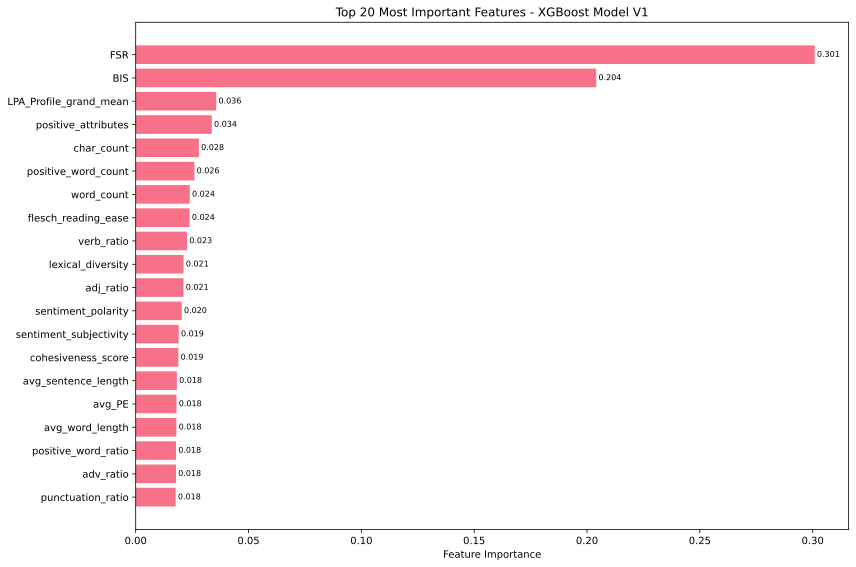
\includegraphics[width=\textwidth]{fig/models/V1/visualizations/feature_importance_v1.pdf}
    \caption{Feature Importance – V1}
    \label{fig:featimp-v1}
\end{subfigure}
\hfill
\begin{subfigure}{0.48\textwidth}
    \centering
    \includegraphics[width=\textwidth]{fig/models/V1/visualizations/characteristic_importance_v1.pdf}
    \caption{Characteristic Importance – V1}
    \label{fig:charimp-v1}
\end{subfigure}

\caption{Top features and characteristic-level contributions for Model V1.}
\label{fig:v1-feat-importance}
\end{figure}

Figure~\ref{fig:v1-feat-importance} shows that FSR emerges as the strongest predictor 
(importance $\approx 0.301$), followed by BIS (importance $\approx 0.204$). Several 
linguistic features—including word count, character count, readability metrics, and 
sentiment polarity—also contribute meaningfully. In contrast, all LLM-derived 
characteristic features receive an importance score of zero, indicating that the 
characteristic extraction pipeline in this version was not functioning as intended.

Taken together, these results highlight the strong predictive power of structured 
behavioral measures and the supplementary value of traditional linguistic features, 
while underscoring the need to refine the LLM-based characteristic extraction 
pipeline in subsequent versions.

% ------------------------------------------------------------------------------------------------------------------------
\subsubsection{Model V2}

%-------------------------------------------------
% classification report for V2
\begin{table}[H]
\centering
\small
\begin{tabular}{l l c c c c}
\toprule
\textbf{Model} & \textbf{Class} & \textbf{Precision} & \textbf{Recall} & \textbf{F1-score} & \textbf{Support} \\
\midrule

\multirow{4}{*}{V2}
 & 0 & 0.835 & 0.840 & 0.837 & 181 \\
 & 1 & 0.906 & 0.904 & 0.905 & 311 \\
 & Macro avg & 0.871 & 0.872 & 0.871 & 492 \\
 & Weighted avg & 0.880 & 0.880 & 0.880 & 492 \\
\bottomrule
\end{tabular}
\caption{Classification report for Model V2.}
\label{tab:v2-classification}
\end{table}

Table~\ref{tab:v2-classification} summarizes the performance of Model V2. Compared to the 
baseline V1, this version incorporates an enhanced characteristic extraction pipeline and a 
scaled feature set. The model achieves balanced and robust performance, with an F1-score of 
0.837 for class~0 and 0.905 for class~1. The macro and weighted averages (0.871 and 0.880) 
indicate that Model~V2 performs consistently across both TD and ASD participants, reflecting 
improvements to both linguistic and characteristic-level representations.

%-------------------------------------------------
% confusion matrix for V2
\begin{table}[H]
\centering
\begin{tabular}{lcc}
\toprule
 & \textbf{Pred 0} & \textbf{Pred 1} \\
\midrule
\textbf{Act 0} & 152 & 29 \\
\textbf{Act 1} & 30 & 281 \\
\bottomrule
\end{tabular}
\caption{Confusion matrix for Model V2.}
\label{tab:v2-confusion}
\end{table}

The confusion matrix in Table~\ref{tab:v2-confusion} shows balanced misclassification rates, 
with 29 false positives and 30 false negatives. Compared to V1, this model preserves strong 
classification performance while benefiting from expanded linguistic and characteristic 
features that refine the representation of participant responses.

%-------------------------------------------------
% Figure 5: Characteristic + Feature Importance (V2)
\begin{figure}[H]
\centering

\begin{subfigure}{0.48\textwidth}
    \centering
    \includegraphics[width=\textwidth]{fig/models/V2/visualizations/characteristic_importance_v2.pdf}
    \caption{Characteristic Importance - V2}
    \label{fig:v2-importance-a}
\end{subfigure}
\hfill
\begin{subfigure}{0.48\textwidth}
    \centering
    \includegraphics[width=\textwidth]{fig/models/V2/visualizations/feature_importance_v2.pdf}
    \caption{Feature Importance - V2)}
    \label{fig:v2-importance-b}
\end{subfigure}

\caption{Characteristic-level contributions and Top Features for Model V2.}
\label{fig:v2-importance}
\end{figure}

Figure~\ref{fig:v2-importance} illustrates how V2 integrates both characteristic-level 
and linguistic-behavioral signals. As shown in Figure~\ref{fig:v2-importance}(a), the 
characteristic extractor contributes meaningful predictive signal, with music, sports, 
personality inference, and arts and crafts emerging as the most influential categories. 
This represents a clear improvement over V1, where all characteristic features had zero 
importance. 

Figure~\ref{fig:v2-importance}(b) highlights the strongest predictors in the model. As in V1, 
FSR remains the most influential feature (importance $\approx 0.312$). However, V2 shows 
substantial gains from characteristic-derived signals such as \textit{music\_positive}, 
\textit{sports\_positive}, and \textit{personality\_inference\_negative}. Traditional 
linguistic features—including word count, character count, readability metrics, and shortness 
score—also continue to contribute meaningfully. 

Overall, the improvements in both characteristic importance and linguistic diversity indicate 
that Model~V2 benefits from a more expressive and well-structured feature extraction pipeline, 
resulting in stronger representations and more balanced predictive performance.

% ------------------------------------------------------------------------------------------------------------------------
\subsubsection{Model V3}

%-------------------------------------------------
% classification report for V3
\begin{table}[H]
\centering
\small
\begin{tabular}{l l c c c c}
\toprule
\textbf{Model} & \textbf{Class} & \textbf{Precision} & \textbf{Recall} & \textbf{F1-score} & \textbf{Support} \\
\midrule

\multirow{4}{*}{V3}
 & 0 & 0.823 & 0.823 & 0.823 & 181 \\
 & 1 & 0.897 & 0.897 & 0.897 & 311 \\
 & Macro avg & 0.860 & 0.860 & 0.860 & 492 \\
 & Weighted avg & 0.871 & 0.871 & 0.871 & 492 \\
\bottomrule
\end{tabular}
\caption{Classification report for Model V3.}
\label{tab:v3-classification}
\end{table}

Model~V3 introduces a more advanced characteristic extraction pipeline using the \textbf{Qwen agent}. 
This represents a key transition from the Sonnet-based system used in V2, enabling richer semantic 
features and improved contextual reasoning in the extracted characteristics. As shown in 
Table~\ref{tab:v3-classification}, the model achieves strong and consistent performance, with 
F1-scores of 0.823 for class~0 and 0.897 for class~1. The macro and weighted averages 
(both 0.860 and 0.871) indicate stable performance across both TD and ASD groups, maintaining parity 
with V2 while benefiting from a more expressive feature set.

%-------------------------------------------------
% confusion matrix for V3
\begin{table}[H]
\centering
\begin{tabular}{lcc}
\toprule
 & \textbf{Pred 0} & \textbf{Pred 1} \\
\midrule
\textbf{Act 0} & 149 & 32 \\
\textbf{Act 1} & 32 & 279 \\
\bottomrule
\end{tabular}
\caption{Confusion matrix for Model V3.}
\label{tab:v3-confusion}
\end{table}

The confusion matrix in Table~\ref{tab:v3-confusion} shows that misclassifications remain balanced 
across classes (32 false positives and 32 false negatives). Despite a slightly larger error count 
than V2, the model retains strong generalization and a stable decision boundary—reflecting improvements 
in the characteristic patterns extracted by Qwen.

%-------------------------------------------------
% Figure: Characteristic + Feature Importance (V3)
\begin{figure}[H]
\centering

\begin{subfigure}{0.48\textwidth}
    \centering
    \includegraphics[width=\textwidth]{fig/models/V3/visualizations/characteristic_importance_v3.pdf}
    \caption{Characteristic Importance -- V3}
    \label{fig:v3-importance-a}
\end{subfigure}
\hfill
\begin{subfigure}{0.48\textwidth}
    \centering
    \includegraphics[width=\textwidth]{fig/models/V3/visualizations/feature_importance_v3.pdf}
    \caption{Feature Importance -- V3}
    \label{fig:v3-importance-b}
\end{subfigure}

\caption{Characteristic-level contributions and Top Features for Model V3.}
\label{fig:v3-importance}
\end{figure}

Figure~\ref{fig:v3-importance}(a) shows that Model~V3 benefits significantly from the upgraded 
Qwen-based characteristic extractor. Music remains the strongest characteristic category 
(importance $\approx 0.099$), followed by food, sweets, personality inference, arts and crafts, 
and sports. Unlike V1---and to a lesser extent V2---all major characteristics now contribute 
non-zero importance, indicating improved semantic grounding and more reliable extraction of 
topic-level patterns within participant responses.

Figure~\ref{fig:v3-importance}(b) presents the top predictive features for V3. As in previous 
models, FSR remains the dominant predictor (importance $\approx 0.282$). However, V3 shows notable 
gains in the contribution of characteristic-derived signals, including \textit{music\_positive}, 
\textit{music\_mentioned}, \textit{food\_mentioned}, and several sentiment-oriented feature variants 
across categories. Traditional linguistic measures---word count, character count, readability, and 
sentence-level attributes---continue to provide complementary value. 

Overall, the introduction of the Qwen agent in Model~V3 enhances the reliability and expressiveness 
of characteristic features, producing a richer feature space and maintaining competitive performance 
ahead of the more advanced LLaMA-based pipeline introduced in later versions.


% ------------------------------------------------------------------------------------------------------------------------
\subsubsection{Model V4}

%-------------------------------------------------
% classification report for V4
\begin{table}[H]
\centering
\small
\begin{tabular}{l l c c c c}
\toprule
\textbf{Model} & \textbf{Class} & \textbf{Precision} & \textbf{Recall} & \textbf{F1-score} & \textbf{Support} \\
\midrule

\multirow{4}{*}{V4}
 & 0 & 0.859 & 0.883 & 0.871 & 180 \\
 & 1 & 0.931 & 0.917 & 0.924 & 311 \\
 & Macro avg & 0.895 & 0.900 & 0.898 & 491 \\
 & Weighted avg & 0.905 & 0.904 & 0.904 & 491 \\
\bottomrule
\end{tabular}
\caption{Classification report for Model V4.}
\label{tab:v4-classification}
\end{table}

Table~\ref{tab:v4-classification} summarizes the performance of Model~V4. This version
introduces a more structured characteristic extraction pipeline based on a Qwen model, an expanded linguistic feature set, and a refined preprocessing
workflow. The model achieves strong and well-balanced performance, with an F1-score of
0.871 for class~0 and 0.924 for class~1. Macro and weighted averages near 0.90 indicate
reliable generalization across both TD and ASD groups. Compared to V3, V4 provides modest
gains in precision and overall consistency.

%-------------------------------------------------
% confusion matrix for V4
\begin{table}[H]
\centering
\begin{tabular}{lcc}
\toprule
 & \textbf{Pred 0} & \textbf{Pred 1} \\
\midrule
\textbf{Act 0} & 159 & 21 \\
\textbf{Act 1} & 26 & 285 \\
\bottomrule
\end{tabular}
\caption{Confusion matrix for Model V4.}
\label{tab:v4-confusion}
\end{table}

The confusion matrix in Table~\ref{tab:v4-confusion} shows that V4 reduces false positives
relative to V3 (21 vs.\ 32), indicating better separation of TD participants. False negatives
remain low (26), reflecting strong ASD detection performance. These results highlight the
stability added by improved preprocessing and more structured characteristic embeddings.

%-------------------------------------------------
% Figure: Characteristic + Feature Importance (V4)
\begin{figure}[H]
\centering

\begin{subfigure}{0.48\textwidth}
    \centering
    \includegraphics[width=\textwidth]{fig/models/V4/visualizations/characteristic_importance_V4.png}
    \caption{Characteristic Importance -- V4}
    \label{fig:v4-importance-a}
\end{subfigure}
\hfill
\begin{subfigure}{0.48\textwidth}
    \centering
    \includegraphics[width=\textwidth]{fig/models/V4/visualizations/feature_importance_V4.png}
    \caption{Feature Importance -- V4}
    \label{fig:v4-importance-b}
\end{subfigure}

\caption{Characteristic-level and feature-level importance distributions for Model~V4.}
\label{fig:v4-importance}
\end{figure}

Figure~\ref{fig:v4-importance} illustrates the contributions of both characteristic-level
and linguistic--behavioral features. In Figure~\ref{fig:v4-importance-a}, food-related
characteristics emerge as the strongest semantic predictors, followed by sports,
personality inference, and music. These patterns indicate that the improved Qwen-based
extractor produces cleaner and more discriminative semantic categories than in earlier
versions.

Figure~\ref{fig:v4-importance-b} shows that FSR remains the dominant predictor
(importance $\approx 0.325$), followed by concise linguistic measures such as
shortness score, character count, and positive/negative food- or sports-related
mentions. Compared to V3, V4 exhibits a more balanced distribution across characteristic
and linguistic dimensions, reflecting enhancements to both the NLP preprocessing and
the characteristic extraction pipeline.

Overall, Model~V4 delivers the strongest performance among the baseline trial-level
models, driven by improved semantic representations, expanded linguistic cues, and a
more stable training workflow.

% ------------------------------------------------------------------------------------------------------------------------
\subsubsection{Model V5}

Model~V5 serves as an ablation study designed to evaluate model performance 
\textit{without} any LLM-derived characteristic features. In contrast to 
Models~V2–V4, which integrate Qwen-based semantic representations, V5 relies 
exclusively on structured behavioral measures (FSR, PE), temporal slope features, 
and classical psycholinguistic attributes extracted through deterministic NLP 
methods. This version isolates the contribution of non-LLM features and assesses 
the extent to which semantic characteristics are necessary for accurate 
classification.

%-------------------------------------------------
% confusion matrix for V5 (if added later)
% \begin{table}[H]
% \centering
% \begin{tabular}{lcc}
% \toprule
%  & \textbf{Pred 0} & \textbf{Pred 1} \\
% \midrule
% \textbf{Act 0} & -- & -- \\
% \textbf{Act 1} & -- & -- \\
% \bottomrule
% \end{tabular}
% \caption{Confusion matrix for Model V5.}
% \label{tab:v5-confusion}
% \end{table}

Cross-validation results indicate strong and stable performance, with a mean 
accuracy of $0.905 \pm 0.015$. These values are comparable to V4, demonstrating 
that the removal of LLM-based characteristics does not significantly degrade 
predictive accuracy. However, the feature distribution shifts substantially, 
revealing the extent to which the model now depends on core behavioral and 
psycholinguistic measures.

%-------------------------------------------------
% Pair of plots (Characteristic importance is empty)
\begin{figure}[H]
\centering

\begin{subfigure}{0.48\textwidth}
    \centering
    \includegraphics[width=\textwidth]{fig/models/V5/visualizations/feature_importance_V5.png}
    \caption{Feature Importance – V5}
    \label{fig:v5-featimp}
\end{subfigure}
\hfill
\begin{subfigure}{0.48\textwidth}
    \centering
    \includegraphics[width=\textwidth]{fig/models/V5/visualizations/feature_importance_by_target_V5.png}
    \caption{Feature Values by Class – V5}
    \label{fig:v5-featimpbyclass}
\end{subfigure}

\caption{Top features and TD/ASD feature comparison for Model~V5.}
\label{fig:v5-importance}
\end{figure}

Figure~\ref{fig:v5-importance}(a) shows the top predictors for V5. With the 
characteristic features removed entirely, the model becomes highly concentrated 
around traditional behavioral measures. \texttt{FSR\_scaled} dominates the 
feature landscape with an importance score of approximately $0.638$, far higher 
than in previous versions. Secondary contributors include lexical diversity, 
shortness score, sentiment polarity, and sentiment subjectivity, each with 
modest but meaningful importance ($0.036$–$0.055$). The temporal slope feature 
\texttt{mean\_slope\_subcat} and scaled PE scores also contribute consistently.

Figure~\ref{fig:v5-importance}(b) displays the average feature values across TD 
and ASD participants. Although the characteristic features are absent, clear 
group-level differences remain in the core features—particularly FSR, where ASD 
participants exhibit substantially higher values.

Overall, Model~V5 demonstrates that the combination of structured behavioral 
measures and traditional psycholinguistic features is sufficient to achieve 
high predictive accuracy, even without LLM-based semantic characteristics. 
However, the extreme reliance on FSR underscores the limited dimensionality of 
the feature space in this ablated configuration, motivating the richer and more 
balanced modeling strategies explored in subsequent versions.


% ------------------------------------------------------------------------------------------------------------------------
\subsubsection{Model V6}

%-------------------------------------------------
% classification report for V6
\begin{table}[H]
\centering
\small
\begin{tabular}{l l c c c c}
\toprule
\textbf{Model} & \textbf{Class} & \textbf{Precision} & \textbf{Recall} & \textbf{F1-score} & \textbf{Support} \\
\midrule

\multirow{4}{*}{V6}
 & 0 & 0.878 & 0.867 & 0.873 & 83 \\
 & 1 & 0.922 & 0.929 & 0.925 & 141 \\
 & Macro avg & 0.900 & 0.898 & 0.899 & 224 \\
 & Weighted avg & 0.904 & 0.906 & 0.905 & 224 \\
\bottomrule
\end{tabular}
\caption{Classification report for Model V6.}
\label{tab:v6-classification}
\end{table}

Table~\ref{tab:v6-classification} summarizes the performance of Model~V6. 
This version intentionally removes all characteristic-derived features. The Qwen-based 
extractor produced near-zero variance across characteristic categories, rendering those 
signals uninformative. As a result, V6 relies exclusively on behavioral and linguistic 
features. Despite this ablation, the model maintains strong performance, achieving 
F1-scores of 0.873 (class~0) and 0.925 (class~1), with a macro-average F1 of 0.899.

%-------------------------------------------------
% confusion matrix for V6
\begin{table}[H]
\centering
\begin{tabular}{lcc}
\toprule
 & \textbf{Pred 0} & \textbf{Pred 1} \\
\midrule
\textbf{Act 0} & 72 & 11 \\
\textbf{Act 1} & 10 & 131 \\
\bottomrule
\end{tabular}
\caption{Confusion matrix for Model V6.}
\label{tab:v6-confusion}
\end{table}

The confusion matrix in Table~\ref{tab:v6-confusion} shows well-balanced error rates, 
with only 11 false positives and 10 false negatives. Model~V6 reliably distinguishes 
between TD and ASD participants using sentence structure, readability, sentiment, 
word/sentence length patterns, and FSR-derived inputs.

%-------------------------------------------------
% Figure: Characteristic + Feature Importance (V6)
\begin{figure}[H]
\centering

\begin{subfigure}{0.48\textwidth}
    \centering
    \includegraphics[width=\textwidth]{fig/models/V6/visualizations/characteristic_importance_V6.png}
    \caption{Characteristic Importance – V6}
    \label{fig:v6-importance-a}
\end{subfigure}
\hfill
\begin{subfigure}{0.48\textwidth}
    \centering
    \includegraphics[width=\textwidth]{fig/models/V6/visualizations/feature_importance_V6.png}
    \caption{Feature Importance – V6}
    \label{fig:v6-importance-b}
\end{subfigure}

\caption{Characteristic-level (left) and feature-level (right) importance for Model V6.}
\label{fig:v6-importance}
\end{figure}

Figure~\ref{fig:v6-importance} highlights a key insight of this version. 
Panel~(a) shows that all characteristic categories receive an importance score of zero, 
confirming the failure of the characteristic extractor for V6. In contrast, 
Panel~(b) shows that the model relies heavily on behavioral and linguistic cues. 
\textit{FSR\_scaled} is the dominant predictor (importance $\approx 0.640$), followed by 
\textit{char\_count}, \textit{word\_count}, \textit{shortness\_score}, 
\textit{avg\_sentence\_length}, and sentiment/readability metrics. These patterns 
align with earlier versions where linguistic structure consistently provides 
strong diagnostic signal.

Overall, Model~V6 serves as a clean behavioral–linguistic baseline. Even without any 
characteristic-level signal, the model achieves strong accuracy (0.906) and stable 
cross-validation performance (mean CV = 0.894 $\pm$ 0.024). This demonstrates the 
robustness of linguistic structure and FSR-derived measures, while highlighting 
the limitations of the Qwen-based characteristic extraction in this configuration.

% ------------------------------------------------------------------------------------------------------------------------
    \subsubsection{Model V7 - With FSR}
    
    
    
    %classification reports for v7-1,2,3
    \begin{table}[H]
    \centering
    \small
    \begin{tabular}{l l c c c c}
    \toprule
    \textbf{Model} & \textbf{Class} & \textbf{Precision} & \textbf{Recall} & \textbf{F1-score} & \textbf{Support} \\
    \midrule
    
    \multirow{4}{*}{V7-1 (Baseline)}
     & 0 & 0.827 & 0.905 & 0.865 & 74 \\
     & 1 & 0.939 & 0.885 & 0.911 & 122 \\
     & Macro avg & 0.883 & 0.895 & 0.888 & 196 \\
     & Weighted avg & 0.897 & 0.893 & 0.894 & 196 \\
    \midrule
    
    \multirow{4}{*}{V7-2}
     & 0 & 0.472 & 1.000 & 0.642 & 312 \\
     & 1 & 0.000 & 0.000 & 0.000 & 348 \\
     & Macro avg & 0.236 & 0.500 & 0.321 & 660 \\
     & Weighted avg & 0.223 & 0.472 & 0.303 & 660 \\
    \midrule
    
    \multirow{4}{*}{V7-3}
     & 0 & 1.000 & 1.000 & 1.000 & 57 \\
     & 1 & 1.000 & 1.000 & 1.000 & 263 \\
     & Macro avg & 1.000 & 1.000 & 1.000 & 320 \\
     & Weighted avg & 1.000 & 1.000 & 1.000 & 320 \\
    \bottomrule
    \end{tabular}
    \caption{Classification reports for models V7-1, V7-2, and V7-3.}
    \label{tab:combined-v7-classification}
    \end{table}
    
    Table~\ref{tab:combined-v7-classification} presents the classification reports for the three V7 
    models, and Table~\ref{tab:v7-confusion} shows the corresponding confusion matrices. 
    Model V7-1, which serves as the baseline, achieves strong and well-balanced performance, 
    with an F1-score of 0.865 for class~0 and 0.911 for class~1. The macro and weighted 
    averages are similarly high (0.888 and 0.894), indicating that the model performs 
    consistently across both classes. The confusion matrix confirms this pattern: the model 
    correctly classifies most samples in each class, misclassifying only a small number of 
    cases (7 false positives and 14 false negatives). These results demonstrate that V7-1 
    captures both TD and ASD patterns effectively and generalizes well.
    
    
    
    %-------------------------------------------------
    %confusion matrix for v7-1,2,3
    \begin{table}[H]
    \centering
    
    \begin{minipage}{0.32\linewidth}
    \centering
    \begin{tabular}{lcc}
    \toprule
     & \textbf{Pred 0} & \textbf{Pred 1} \\
    \midrule
    \textbf{Act 0} & 67 & 7 \\
    \textbf{Act 1} & 14 & 108 \\
    \bottomrule
    \end{tabular}
    \caption*{V7-1 (Baseline)}
    \end{minipage}
    \hfill
    \begin{minipage}{0.32\linewidth}
    \centering
    \begin{tabular}{lcc}
    \toprule
     & \textbf{Pred 0} & \textbf{Pred 1} \\
    \midrule
    \textbf{Act 0} & 312 & 0 \\
    \textbf{Act 1} & 348 & 0 \\
    \bottomrule
    \end{tabular}
    \caption*{V7-2}
    \end{minipage}
    \hfill
    \begin{minipage}{0.32\linewidth}
    \centering
    \begin{tabular}{lcc}
    \toprule
     & \textbf{Pred 0} & \textbf{Pred 1} \\
    \midrule
    \textbf{Act 0} & 57 & 0 \\
    \textbf{Act 1} & 0 & 263 \\
    \bottomrule
    \end{tabular}
    \caption*{V7-3}
    \end{minipage}
    
    \caption{Confusion matrices for models V7-1, V7-2, and V7-3.}
    \label{tab:v7-confusion}
    \end{table}
    
    In contrast, Model V7-2 exhibits highly unbalanced behavior. While it classifies every 
    instance of class~0 correctly (precision and recall of 1.0), it fails entirely on class~1, 
    predicting none of the positive samples correctly. This extreme skew is evident in the 
    confusion matrix, where all 348 class~1 instances are predicted as class~0. The macro-average 
    F1-score drops to 0.321, and the weighted F1-score falls to 0.303. This behavior indicates 
    that when the test data are restricted to the FSR-overlapped region, the model becomes biased 
    toward the negative class, suggesting that the distribution shift or reduced feature diversity 
    severely impacts the model’s ability to recognize class~1 patterns.
    
    Model V7-3 shows the opposite behavior: both classes achieve perfect precision, recall, and 
    F1-score (1.0). The confusion matrix likewise shows no misclassifications. However, this 
    apparent perfection must be interpreted cautiously. V7-3 is trained only on the FSR-overlapped 
    region, which is substantially smaller and much more homogeneous than the full dataset. The 
    perfect scores therefore reflect overfitting to a highly constrained training distribution, 
    rather than true generalization. Although the model performs flawlessly on its evaluation 
    subset, it likely lacks robustness when applied beyond the restricted region. Together, the 
    results from V7-2 and V7-3 highlight the sensitivity of the model to training–testing 
    distribution alignment, and they underscore the importance of using the full, balanced 
    dataset for reliable model performance.
    
    
    %-------------------------------------------------
    %feature importance plots
    \begin{figure}[H]
    \centering
    
    \begin{subfigure}{0.32\textwidth}
        \centering
        \includegraphics[width=\textwidth]{fig/models/V7-1/visualizations/feature_importance_V7-1.png}
        \caption{V7-1}
        \label{fig:featimp-v7-1}
    \end{subfigure}
    \hfill
    \begin{subfigure}{0.32\textwidth}
        \centering
        \includegraphics[width=\textwidth]{fig/models/V7-2/visualizations/feature_importance_V7-2.png}
        \caption{V7-2}
        \label{fig:featimp-v7-2}
    \end{subfigure}
    \hfill
    \begin{subfigure}{0.32\textwidth}
        \centering
        \includegraphics[width=\textwidth]{fig/models/V7-3/visualizations/feature_importance_V7-3.png}
        \caption{V7-3}
        \label{fig:featimp-v7-3}
    \end{subfigure}
    
    \caption{Comparison of Feature Importance Across Models V7-1, V7-2, V7-3}
    \label{fig:featimp-v7-comparison}
    \end{figure}
    
    Figure~\ref{fig:featimp-v7-comparison} compares the top features across models V7-1, V7-2, and V7-3. 
    Across all three models, FSR consistently emerges as the most dominant predictor by a large margin, 
    indicating its strong influence on ASD versus TD classification. However, the relative contributions 
    of the remaining features differ substantially across models, reflecting the impact of training and 
    testing region choices. In V7-1, the importance scores are more evenly distributed, with linguistic 
    features such as word count, lexical diversity, sentiment subjectivity, and readability metrics 
    contributing meaningfully alongside the PE-based measures. By contrast, V7-2 displays a highly 
    skewed profile in which FSR alone accounts for nearly half of the total importance, while most other 
    features contribute minimally. This pattern is consistent with the model's poor performance on class~1 
    and suggests that the restricted evaluation region amplifies the reliance on a single dominant signal. 
    The V7-3 model, trained exclusively on the overlapped region, shows a more balanced distribution than 
    V7-2 but still places disproportionate weight on FSR. Although many linguistic and concept-learning 
    features regain moderate influence in V7-3, their relative importance remains lower than in V7-1. 
    Taken together, these results indicate that while FSR is consistently the strongest feature, the 
    diversity and stability of secondary predictors degrade when the model is trained or evaluated on 
    restricted subsets of the data, reinforcing the importance of using the full dataset for capturing 
    richer linguistic and behavioral patterns.
    
    %-------------------------------------------------
    %feature importance by targets plots
    \begin{figure}[H]
    \centering
    
    \begin{subfigure}{0.32\textwidth}
        \centering
        \includegraphics[width=\textwidth]{fig/models/V7-1/visualizations/feature_importance_by_target_V7-1.png}
        \caption{V7-1}
        \label{fig:featimpbytar-v7-1}
    \end{subfigure}
    \hfill
    \begin{subfigure}{0.32\textwidth}
        \centering
        \includegraphics[width=\textwidth]{fig/models/V7-2/visualizations/feature_importance_by_target_V7-2.png}
        \caption{V7-2}
        \label{fig:featimpbytar-v7-2}
    \end{subfigure}
    \hfill
    \begin{subfigure}{0.32\textwidth}
        \centering
        \includegraphics[width=\textwidth]{fig/models/V7-3/visualizations/feature_importance_by_target_V7-3.png}
        \caption{V7-3}
        \label{fig:featimpbytar-v7-3}
    \end{subfigure}
    
    \caption{Comparison of Feature Importance By Target Models V7-1, V7-2, V7-3}
    \label{fig:featimpbytar-v7-comparison}
    \end{figure}
    
    Figure~\ref{fig:featimpbytar-v7-comparison} compares not only the feature importance rankings but 
    also the average feature values between TD and ASD participants across models V7-1, V7-2, and 
    V7-3. Across all three models, FSR remains the most influential feature and also shows the 
    largest separation between the two groups, with ASD participants consistently exhibiting 
    substantially higher FSR scores. Several linguistic features also display meaningful group 
    differences. For example, ASD responses tend to be longer, reflected in higher word count 
    and character count values, while TD responses generally score higher on readability metrics 
    such as Flesch reading ease. Additional differences appear in sentiment- and lexicon-based 
    features: ASD participants often produce more negative words and lower sentiment polarity, 
    whereas TD participants typically show slightly higher lexical diversity. Although the 
    magnitude of these differences varies across models, the overall pattern remains consistent. 
    When comparing the models, V7-1 presents the richest and most balanced feature contributions, 
    with several linguistic and cognitive features showing clear class separation. V7-2 compresses 
    most differences except for FSR, consistent with its over-reliance on a single dominant signal, 
    while V7-3 restores some of the class distinctions but still exhibits reduced variability 
    relative to V7-1. Taken together, these plots highlight that both linguistic style and 
    cognitive performance metrics contribute to distinguishing ASD from TD responses, with FSR 
    serving as the strongest and most stable predictor across all settings.

% ------------------------------------------------------------------------------------------------------------------------

\subsubsection{Model V8 - Without FSR}

%-------------------------------------------------
%classification reports for v8-1,2,3
\begin{table}[H]
\centering
\small
\begin{tabular}{l l c c c c}
\toprule
\textbf{Model} & \textbf{Class} & \textbf{Precision} & \textbf{Recall} & \textbf{F1-score} & \textbf{Support} \\
\midrule

\multirow{4}{*}{V8-1 (Baseline)}
 & 0 & 0.509 & 0.378 & 0.434 & 74 \\
 & 1 & 0.674 & 0.779 & 0.722 & 122 \\
 & Macro avg & 0.591 & 0.579 & 0.578 & 196 \\
 & Weighted avg & 0.612 & 0.628 & 0.614 & 196 \\
\midrule

\multirow{4}{*}{V8-2}
 & 0 & 0.525 & 0.099 & 0.167 & 312 \\
 & 1 & 0.532 & 0.919 & 0.674 & 348 \\
 & Macro avg & 0.529 & 0.509 & 0.421 & 660 \\
 & Weighted avg & 0.529 & 0.532 & 0.435 & 660 \\
\midrule

\multirow{4}{*}{V8-3}
 & 0 & 0.286 & 0.596 & 0.386 & 57 \\
 & 1 & 0.885 & 0.677 & 0.767 & 263 \\
 & Macro avg & 0.586 & 0.637 & 0.577 & 320 \\
 & Weighted avg & 0.778 & 0.663 & 0.699 & 320 \\
\bottomrule
\end{tabular}
\caption{Classification reports for models V8-1, V8-2, and V8-3.}
\label{tab:v8-classification}
\end{table}

Table~\ref{tab:v8-classification} and Table~\ref{tab:v8-confusions} present the performance 
of models V8-1, V8-2, and V8-3, which rely solely on PE-derived features and concept-learning 
scores, without using FSR. Across all three models, performance is noticeably lower than 
their V7 counterparts, confirming that removing FSR eliminates the strongest predictive 
signal. V8-1, the baseline configuration, shows moderate but balanced performance, with close 
precision and recall values for both classes and a weighted F1-score of 0.614. The confusion 
matrix indicates that V8-1 misclassifies a substantial number of samples from both classes, 
although it retains some discriminative ability.



%-------------------------------------------------
%confusion matrix for v8-1,2,3
\begin{table}[H]
\centering

\begin{minipage}{0.32\linewidth}
\centering
\begin{tabular}{lcc}
\toprule
 & \textbf{Pred 0} & \textbf{Pred 1} \\
\midrule
\textbf{Act 0} & 28 & 46 \\
\textbf{Act 1} & 27 & 95 \\
\bottomrule
\end{tabular}
\caption*{V8-1 (Baseline)}
\end{minipage}
\hfill
\begin{minipage}{0.32\linewidth}
\centering
\begin{tabular}{lcc}
\toprule
 & \textbf{Pred 0} & \textbf{Pred 1} \\
\midrule
\textbf{Act 0} & 31 & 281 \\
\textbf{Act 1} & 28 & 320 \\
\bottomrule
\end{tabular}
\caption*{V8-2}
\end{minipage}
\hfill
\begin{minipage}{0.32\linewidth}
\centering
\begin{tabular}{lcc}
\toprule
 & \textbf{Pred 0} & \textbf{Pred 1} \\
\midrule
\textbf{Act 0} & 34 & 23 \\
\textbf{Act 1} & 85 & 178 \\
\bottomrule
\end{tabular}
\caption*{V8-3}
\end{minipage}

\caption{Confusion matrices for models V8-1, V8-2, and V8-3.}
\label{tab:v8-confusions}
\end{table}

V8-2 improves recall substantially for class~1 (0.919) but at the cost of very low recall 
for class~0 (0.099), resulting in a highly asymmetric prediction pattern. The confusion 
matrix reflects this imbalance: the model predicts almost all samples as class~1, capturing 
most ASD cases but failing to correctly identify TD participants. This behavior suggests 
that certain PE-derived features strongly correlate with ASD but offer limited information 
for distinguishing TD.

V8-3 presents a more balanced profile than V8-2, achieving higher recall for class~1 
(0.767) while retaining moderate recall for class~0 (0.596). The weighted F1-score (0.592) 
is the highest among the V8 models. The confusion matrix shows fewer extreme misclassifications 
compared to V8-2, indicating better generalization across both groups. Overall, the V8 
results demonstrate that PE-normalized features and concept-learning metrics carry meaningful 
signal for ASD detection, but their predictive power is considerably weaker without FSR. 
The differences among V8-1, V8-2, and V8-3 highlight the sensitivity of model performance 
to specific subsets of PE-related features, as well as the challenges of maintaining balanced 
class discrimination when the dominant feature is removed.

%-------------------------------------------------
%feature importance plots
\begin{figure}[H]
\centering

\begin{subfigure}{0.32\textwidth}
    \centering
    \includegraphics[width=\textwidth]{fig/models/V8-1/visualizations/feature_importance_V8-1.png}
    \caption{V8-1}
    \label{fig:featimp-v8-1}
\end{subfigure}
\hfill
\begin{subfigure}{0.32\textwidth}
    \centering
    \includegraphics[width=\textwidth]{fig/models/V8-1/visualizations/feature_importance_V8-1.png}
    \caption{V8-2}
    \label{fig:featimp-v8-2}
\end{subfigure}
\hfill
\begin{subfigure}{0.32\textwidth}
    \centering
    \includegraphics[width=\textwidth]{fig/models/V8-1/visualizations/feature_importance_V8-1.png}
    \caption{V8-3}
    \label{fig:featimp-v8-3}
\end{subfigure}

\caption{Comparison of Feature Importance Across Models V8-1, V8-2, V8-3}
\label{fig:featimp-v8-comparison}
\end{figure}

Figure~\ref{fig:featimp-v8-comparison} compares the top twenty features across models V8-1, V8-2, 
and V8-3. Unlike the V7 series, no single feature dominates across all V8 models, reflecting the 
removal of FSR and the resulting shift toward a more evenly distributed importance profile. 
Across all three models, character count, word count, shortness score, lexical diversity, and 
sentence-level metrics emerge as consistently influential features. However, each model weights 
these features differently. V8-1 shows a relatively balanced spread across character count, 
shortness score, and TDNorm-based PE measures, suggesting that it relies on a broad combination 
of linguistic and cognitive indicators. V8-2 places the highest weight on shortness score and 
word count, which aligns with its asymmetric prediction behavior that favors class~1. Meanwhile, 
V8-3 produces a more uniform distribution of importance scores, where no feature exceeds 0.073, 
suggesting that this model disperses its reliance across multiple linguistic characteristics. 
Taken together, these results indicate that once FSR is removed, the predictive structure of the 
models becomes less centralized and more dependent on general response length, lexical richness, 
and sentence complexity.


%-------------------------------------------------
%feature importance by targets plots
\begin{figure}[H]
\centering

\begin{subfigure}{0.32\textwidth}
    \centering
    \includegraphics[width=\textwidth]{fig/models/V8-1/visualizations/feature_importance_by_target_V8-1.png}
    \caption{V8-1}
    \label{fig:featimpbytar-v8-1}
\end{subfigure}
\hfill
\begin{subfigure}{0.32\textwidth}
    \centering
    \includegraphics[width=\textwidth]{fig/models/V8-2/visualizations/feature_importance_by_target_V8-2.png}
    \caption{V8-2}
    \label{fig:featimpbytar-v8-2}
\end{subfigure}
\hfill
\begin{subfigure}{0.32\textwidth}
    \centering
    \includegraphics[width=\textwidth]{fig/models/V8-3/visualizations/feature_importance_by_target_V8-3.png}
    \caption{V8-3}
    \label{fig:featimpbytar-v8-3}
\end{subfigure}

\caption{Comparison of Feature Importance By Target Models V8-1, V8-2, V8-3}
\label{fig:featimpbytar-v8-comparison}
\end{figure}


Figure~\ref{fig:featimpbytar-v8-comparison} further examines the V8 models by comparing their most 
important features with the underlying class-wise feature distributions. Although the relative 
importance rankings differ across V8-1, V8-2, and V8-3, several systematic differences between 
the TD and ASD groups appear consistently. ASD participants tend to produce shorter but denser 
responses, reflected in lower shortness scores and lower readability scores, but also in higher 
character and word counts in some models, suggesting more compact phrasing or reduced syntactic 
structure. TD participants typically display slightly higher lexical diversity and higher 
readability scores, indicating more varied vocabulary and clearer sentence construction. 
Differences in PE-related measures such as TDNorm\_avg\_PE and overall\_avg\_PE are also present, 
but these are smaller compared to the linguistic distinctions. Across all three models, the class 
distributions provide insight into why certain features become predictive: features that show 
consistent separation between groups, such as sentence length, lexical diversity, and reading ease, 
are repeatedly ranked as important. These patterns highlight that even without FSR, the models 
capture meaningful linguistic tendencies associated with ASD, though the discriminative strength 
of these features is weaker and more diffuse than in the V7 models.



% ------------------------------------------------------------------------------------------------------------------------


\subsection{Clustering Results}

\subsubsection{Consensus Heatmaps}

\begin{figure}[H]
\centering

\begin{subfigure}{0.32\textwidth}
    \centering
    \includegraphics[width=\textwidth]{fig/clustering/V1/plots/consensus_matrix_k4.pdf}
    \caption{K=4}
    \label{fig:ConsensusHeatmap4}
\end{subfigure}
\hfill
\begin{subfigure}{0.32\textwidth}
    \centering
    \includegraphics[width=\textwidth]{fig/clustering/V1/plots/consensus_matrix_k5.pdf}
    \caption{K=5}
    \label{fig:ConsensusHeatmap5}
\end{subfigure}
\hfill
\begin{subfigure}{0.32\textwidth}
    \centering
    \includegraphics[width=\textwidth]{fig/clustering/V1/plots/consensus_matrix_k12.pdf}
    \caption{K=12}
    \label{fig:ConsensusHeatmap12}
\end{subfigure}

\caption{Consensus Matrix for K=4,5 and 12}
\label{fig:ConsensusHeatmapComparison}
\end{figure}

Visual inspection of the consensus matrices, in Figure\ref{fig:ConsensusHeatmapComparison} highlights a clear improvement in cluster separation when moving from k = 4 to k = 5. At k = 4, several large blocks show partial mixing, with broad regions of intermediate consensus values that indicate instability and inconsistent co-assignment across bootstrap runs. The cluster boundaries are diffuse, suggesting that the four-cluster solution is forcing together subgroups that do not consistently co-occur. In contrast, the k = 5 matrix exhibits sharply defined, high-consensus blocks with darker separation bands, reflecting much more stable and internally coherent clusters. The fifth cluster resolves a previously heterogeneous region into a clean, well-supported block, reducing within-cluster variance and improving interpretability. Overall, the consensus heatmaps visually reinforce that k = 5 produces the most stable, well-differentiated set of ASD subgroups


\subsubsection{Best K Selection}

\begin{figure}[H]
\centering

% ---------- Row 1 ----------
\begin{subfigure}{0.32\textwidth}
    \centering
    \includegraphics[width=\textwidth]{fig/clustering/V1/plots/consensus_cdf.pdf}
    \caption{CDF Curves for K Values}
    \label{fig:consensuscdf}
\end{subfigure}
\hfill
\begin{subfigure}{0.32\textwidth}
    \centering
    \includegraphics[width=\textwidth]{fig/clustering/V1/plots/consensus_auc_cdf.pdf}
    \caption{Area Under CDF Curve}
    \label{fig:consensusauc}
\end{subfigure}
\hfill
\begin{subfigure}{0.32\textwidth}
    \centering
    \includegraphics[width=\textwidth]{fig/clustering/V1/plots/consensus_delta_cdf.pdf}
    \caption{Delta of Area Under CDF Curve}
    \label{fig:consensusdeltaauc}
\end{subfigure}

\vspace{0.4cm}

% ---------- Row 2 ----------
\begin{subfigure}{0.32\textwidth}
    \centering
    \includegraphics[width=\textwidth]{fig/clustering/V1/plots/consensus_stability_curve.pdf}
    \caption{Stability Curve}
    \label{fig:consensusstability}
\end{subfigure}
\hfill
\begin{subfigure}{0.32\textwidth}
    \centering
    \includegraphics[width=\textwidth]{fig/clustering/V1/plots/consensus_PAC_curve.pdf}
    \caption{Proportion of Ambiguous Clustering Curve}
    \label{fig:consensuspac}
\end{subfigure}
\hfill
\begin{subfigure}{0.32\textwidth}
    \centering
    % Empty placeholder for spacing
    \vspace{0pt}
\end{subfigure}

\caption{Best K Selection Plots}
\label{fig:BestKSelectionPlots}
\end{figure}

From Figure\ref{fig:BestKSelectionPlots} we can see that we have some potential Best K options: K=4 and K=5. Going off the PAC methodology of best cluster selection, K=5 was chosen as the True number of Clusters present in the ASD only Data. We can also see that the stability curve also indicates K=5 as it is at its peak at that value.

\subsubsection{Cluster Validation and Feature Profiles}

\begin{figure}[H]
\centering

% ---------- Top: 1×1 ----------
\begin{subfigure}{0.9\textwidth}
    \centering
    \includegraphics[width=\textwidth]{fig/clustering/V1/significance_tests/significance.pdf}
    \caption{Overall Significance Test}
\end{subfigure}

\vspace{0.6cm}

% ---------- Bottom: 2×2 ----------
\begin{subfigure}{0.48\textwidth}
    \centering
    \includegraphics[width=\textwidth]{fig/clustering/V1/significance_tests/dunn_FSR.pdf}
    \caption{Significance Test of FSR}
\end{subfigure}
\hfill
\begin{subfigure}{0.48\textwidth}
    \centering
    \includegraphics[width=\textwidth]{fig/clustering/V1/significance_tests/dunn_overall_concept_learning.pdf}
    \caption{Significance Test of overall\_concept\_learning}
\end{subfigure}

\vspace{0.4cm}

\begin{subfigure}{0.48\textwidth}
    \centering
    \includegraphics[width=\textwidth]{fig/clustering/V1/significance_tests/dunn_TDNorm_avg_PE.pdf}
    \caption{Significance Test of TDNorm\_avg\_PE}
\end{subfigure}
\hfill
\begin{subfigure}{0.48\textwidth}
    \centering
    \includegraphics[width=\textwidth]{fig/clustering/V1/significance_tests/dunn_TDnorm_concept_learning.pdf}
    \caption{Significance Test of TDNorm\_concept\_learning}
\end{subfigure}

\caption{Significance Tests}
\label{fig:combined_significance}
\end{figure}



\begin{figure}[H]
\centering

\begin{subfigure}{0.48\textwidth}
    \centering
    \includegraphics[width=\textwidth]{fig/clustering/V1/cluster_profiles/profile_FSR.pdf}
    \caption{Cluster Profile of FSR}
\end{subfigure}
\hfill
\begin{subfigure}{0.48\textwidth}
    \centering
    \includegraphics[width=\textwidth]{fig/clustering/V1/cluster_profiles/profile_overall_concept_learning.pdf}
    \caption{Cluster Profile of overall\_concept\_learning}
\end{subfigure}

\vspace{0.4cm}

\begin{subfigure}{0.48\textwidth}
    \centering
    \includegraphics[width=\textwidth]{fig/clustering/V1/cluster_profiles/profile_TDNorm_avg_PE.pdf}
    \caption{Cluster Profile of TDNorm\_avg\_PE}
\end{subfigure}
\hfill
\begin{subfigure}{0.48\textwidth}
    \centering
    \includegraphics[width=\textwidth]{fig/clustering/V1/cluster_profiles/profile_TDnorm_concept_learning.pdf}
    \caption{Cluster Profile of TDNorm\_concept\_learning}
\end{subfigure}

\caption{Cluster Profiles}
\label{fig:combined_profiles}
\end{figure}


From Figure\ref{fig:combined_significance} we can see that the Dunn post-hoc comparisons further validate that the K = 5 solution yields meaningfully distinct ASD subgroups. For all clinical features used, FSR, overall\_concept\_learning, TDNorm\_avg\_PE, and TDNorm\_concept\_learning—the majority of pairwise cluster comparisons produced very small p-values (often < 0.01 or < 0.001), indicating that specific clusters differ significantly from one another on these dimensions. Only a small number of pairs showed non-significant differences, which is expected when certain clusters share partially overlapping behavioral profiles. Overall, the pattern of pairwise significance demonstrates that the clusters are not only globally different (as shown by ANOVA/Kruskal) but also separately differentiated at the subgroup level, reinforcing that the five-cluster structure captures nuanced, interpretable variability within the ASD population.


\subsubsection{TD Contamination}

\begin{figure}[H]
    \centering
    \includegraphics[width=0.9\textwidth]{fig/clustering/V1/TD_Contamination_Report.pdf}
    \caption{TD Contamination Report}
    \label{fig:TDContam}
\end{figure}



The TD contamination analysis provides insight into how uniquely ASD-specific each consensus cluster is. Two clusters—Cluster 1 and Cluster 3—show extremely low TD fractions (appx.1\% and 3\%), indicating they represent highly ASD-distinct behavioral profiles with minimal overlap from typically developing participants. Cluster 2 and Cluster 0 exhibit moderate contamination (appx.30\% and 38\%), suggesting these groups capture more mixed behavioral patterns that share some similarities with TD profiles. Cluster 4 shows the highest TD fraction (appx.62\%), reflecting a cluster whose behavioral signatures overlap substantially with TD participants and may represent a milder or more compensated ASD phenotype. Overall, the contamination patterns reinforce that the consensus solution captures a spectrum of ASD subtypes, ranging from strongly ASD-specific clusters to those with partial or substantial resemblance to TD behavioral patterns.


% ------------------------------------------------------------------------------------------------------------------------

\section{Conclusions}

\paragraph{Modeling}


Across all model iterations, the results clearly demonstrate that feature composition—and, in particular, the presence or absence of FSR—plays a pivotal role in shaping predictive accuracy, stability, and interpretability in ASD–TD classification. The progression from Models V1 through V6 illustrates a systematic refinement of both the modeling strategy and the underlying feature representations. Early models (V1--V2) revealed that while broad, high-dimensional feature sets can capture rich behavioral and linguistic variability, they also introduce risks of overfitting. Subsequent iterations (V3--V4) benefited substantially from integrating Qwen-derived linguistic features, which provided more discriminative semantic cues and contributed to the strongest overall baseline performance observed in V4. Ablation-focused models (V5--V6) further clarified the central role of structured behavioral metrics and classical linguistic cues, showing that these features alone can sustain strong performance even in the absence of LLM-based characteristics.

Overall, the V7 models substantially outperform the V8 models in both predictive accuracy 
and stability. The strong performance of V7 is driven largely by the inclusion of FSR, which 
consistently emerges as the most discriminative feature and provides a clear cluster boundary 
between TD and ASD participants. Linguistic and concept-learning features complement FSR and 
contribute additional signal, resulting in balanced precision, recall, and generalization in 
the baseline V7-1 model. Even though V7-2 and V7-3 exhibit distribution-related issues when 
trained or tested on restricted subsets, the overall feature structure remains strong.

In contrast, the V8 models show weaker and less stable performance because they rely solely on 
linguistic and PE-derived features without FSR. Without the dominant predictive signal, the 
models depend on many smaller and more diffuse features such as character count, shortness 
score, lexical diversity, and readability metrics. These features still capture meaningful 
differences between TD and ASD groups, but their combined discriminative power is noticeably 
lower. As a result, V8 models show reduced accuracy, higher misclassification rates, and greater 
sensitivity to class imbalance. Taken together, the comparison shows that linguistic and 
cognitive features are informative but insufficient on their own, and that FSR plays a 
crucial role in achieving reliable ASD detection.

\paragraph{Clustering}

In summary, the consensus clustering framework revealed a robust and interpretable five-cluster structure within the ASD cohort, supported by multiple lines of statistical and visual evidence. PAC and stability analyses identified k = 5 as the point where gains in cluster reliability stabilized, and the corresponding consensus matrix displayed sharply defined high-agreement blocks indicative of strong internal cohesion. Across all behavioral and performance features, both one-way ANOVA and Kruskal–Wallis tests demonstrated highly significant differences between clusters, with Dunn post-hoc comparisons further clarifying the specific subgroup distinctions. TD contamination results confirmed that several clusters capture ASD-specific behavioral signatures with minimal overlap from typically developing participants. Together, these findings show that the five-cluster solution captures meaningful heterogeneity within the ASD population, offering a stable and interpretable set of behavioral subtypes that can inform downstream modeling, characterization, and potential clinical insights.

% ------------------------------------------------------------------------------------------------------------------------

\section{Future Work}

Several directions can further extend and strengthen the findings of this study. First, additional validation should be conducted by testing the modeling and clustering frameworks on external datasets. Evaluating the Generalized Detection Model against independent samples would enable a more rigorous assessment of its robustness, generalizability, and sensitivity to population-level variability. Incorporating heterogeneous datasets—such as those differing in age range, linguistic backgrounds, or task structure—would also provide deeper insight into the model’s ability to detect ASD–TD distinctions under a wide range of conditions.

Another additional work is  expanding the clustering analysis to include the entire participant pool. While the current study focuses primarily on task-specific or feature-specific subsets, applying unsupervised methods to the full dataset may reveal broader behavioral–linguistic subgroups, latent participant profiles, or emergent ASD subtypes. Such an approach may uncover macro-level cluster formations that remain hidden when examining limited feature spaces or constrained sample partitions.

Finally, integrating explainable AI (xAI) methods more deeply into the clustering pipeline represents an important future direction. By combining cluster assignments with techniques such as SHAP explanations, counterfactual analysis, or feature-interaction visualizations, future work can provide clearer interpretations of why individuals cluster together and which behavioral or linguistic features drive group separation. This integrated framework would enhance interpretability, support hypothesis generation in developmental research, and ultimately contribute to more transparent and equitable computational models for ASD detection and understanding.






\bibliographystyle{IEEEtran}
\bibliography{references}



\end{document} 